\documentclass[11pt,a4paper]{article}
\usepackage[T1]{fontenc}
\usepackage[utf8]{inputenc}
\usepackage[spanish,es-noshorthands,es-nodecimaldot]{babel}
\usepackage{lmodern,amsmath,amssymb,amsthm,bm}
\usepackage{geometry,graphicx,booktabs,longtable,tabularx,array,float,xcolor}
\usepackage{hyperref,xurl,fancyhdr,listings}
\geometry{margin=2.2cm}
\hypersetup{colorlinks=true,linkcolor=blue!50!black,urlcolor=blue!50!black}
\newtheorem{proposicion}{Proposición}
\newtheorem{observacion}{Observación}
\newcommand{\archivo}[1]{\path{#1}}
\newcommand{\vect}[1]{\bm{#1}}
\newcommand{\R}{\mathbb R}
\lstset{language=Matlab,basicstyle=\ttfamily\small,breaklines=true,frame=single,columns=fullflexible,showstringspaces=false}
\setlength{\parskip}{5pt}
\setlength{\parindent}{0pt}
\setlength{\emergencystretch}{3em}
\pagestyle{fancy}
\fancyhf{}
\fancyhead[L]{VCSEL + lente común + un PD}
\fancyhead[R]{Estudio MATLAB}
\fancyfoot[C]{\thepage}
\setlength{\headheight}{14pt}
\graphicspath{{../resultados/full_20260913_190744_155/figuras/}}
\newcommand{\DirectorioResultados}{\path{resultados/full_20260913_190744_155}}
\newcommand{\NumeroCasos}{25}
\newcommand{\NumeroEnsayos}{7500}
\newcommand{\NumeroSensibilidad}{3200}
\newcommand{\NumeroPruebas}{27}
\newcommand{\TilePdos}{1.31}
\newcommand{\TilePtres}{11.7}
\newcommand{\TileFrontera}{16.2}
\newcommand{\ParFrontera}{382}
\newcommand{\GridPdos}{1.12}
\newcommand{\GridPtres}{11}
\newcommand{\GridFrontera}{9.02}
\newcommand{\TileNovenoPtres}{1.46e+03}
\newcommand{\GridOriginalPtres}{4.27e+03}
\newcommand{\GananciaLibrePtres}{904}

\title{Posicionamiento óptico 2D y 3D con un array de VCSELs, una lente común y un único fotodiodo\\[0.4em]\large Desarrollo matemático, implementación MATLAB y evaluación reproducible}
\author{Estudio computacional basado en la arquitectura de Kazemi}
\date{Versión MATLAB: septiembre de 2026}
\begin{document}
\maketitle
\begin{abstract}
Se plantea y evalúa la recuperación de la posición de un único fotodiodo a partir de potencias individualmente identificadas de un array $5\times5$ de VCSELs. El modelo conserva el acoplamiento entre curvatura de una lente común, refracción de cada emisor y transformación Gaussian mediante matrices ABCD. Se distinguen identificabilidad, estabilidad bajo ruido, convergencia del estimador y validez de las aproximaciones ópticas. La implementación MATLAB se contrasta con valores deterministas de la versión Python y vuelve a ejecutar los experimentos: \NumeroCasos{} casos, \NumeroEnsayos{} localizaciones aleatorias y \NumeroSensibilidad{} pruebas de sensibilidad. Una focal basta en una región local con radiometría y orientación calibradas; dos focales amplían ciertas regiones, pero no garantizan cobertura de todo el volumen nominal. Las variantes más agresivas muestran discrepancias importantes con un trazado independiente de rayos. Este documento explica el razonamiento, las demostraciones bajo sus hipótesis, los experimentos favorables y desfavorables, y la localización de cada archivo necesario para reproducirlos.
\end{abstract}
\textbf{Resultado computacional, no certificación experimental.} Las precisiones indicadas suponen el modelo declarado y no representan mediciones de una lente comercial ni una certificación de seguridad ocular.
\tableofcontents
\clearpage
\section{Planteamiento, objetivos y recorrido del estudio}
\subsection{La pregunta que resolvemos}
El punto de partida es el manuscrito de Hossein Kazemi y colaboradores, \emph{A Novel Terabit Grid-of-Beam Optical Wireless Multi-User Access Network with Beam Clustering}. La fuente disponible es \archivo{../A Novel Terabit Grid-of-Beam Optical/Hossein_TCOM_Final_arXiv.tex}, respecto de la carpeta raíz de este estudio. Se utilizan especialmente las secciones de propagación Gaussian, diseño del transmisor y parámetros numéricos. No se atribuyen al nuevo receptor las ganancias del ADR del artículo.

Para un tile, 25 VCSELs comparten una lente. Su posición dentro del array hace que la lente refracte sus ejes hacia direcciones diferentes. En un estado óptico $k$, el receptor obtiene un vector etiquetado
\begin{equation}
\vect P_k(\vect p)=[P_{1,k}(\vect p),\ldots,P_{25,k}(\vect p)]^T,
\qquad \vect p=[x,y,z]^T.
\end{equation}
Con $K$ estados, la observación es
\begin{equation}\label{eq:observation}
\vect y(\vect p)=[\vect P_1^T,\ldots,\vect P_K^T]^T\in\R^{25K}.
\end{equation}
La identificación por pilotos o encendido secuencial es esencial: no se sustituye este vector por una potencia total. Para el AP completo se conserva la identidad de los 225 emisores y el vector tiene $225K$ componentes.

\textbf{Caso 2D:} se conoce $z=z_0$ y se estiman $(x,y)$. En los experimentos principales $z_0=0$. \textbf{Caso 3D:} se estiman las tres coordenadas. La normal del PD se mantiene conocida; no se considera resuelto un problema conjunto de posición y actitud desconocidas.

\subsection{Qué significa que una solución funcione}
Se separan cuatro preguntas que no son equivalentes:
\begin{enumerate}
\item \textbf{Identificabilidad local:} ¿hay cambios independientes de las potencias frente a las coordenadas?
\item \textbf{Estabilidad:} ¿son esos cambios suficientemente grandes frente al ruido disponible?
\item \textbf{Estimación:} ¿un algoritmo sin la posición verdadera como inicialización encuentra una solución precisa?
\item \textbf{Adecuación física:} ¿la aproximación de haz sigue siendo válida en los estados focales ensayados?
\end{enumerate}
Tener 25 o 225 canales no responde por sí solo a estas preguntas. Un punto puede recibir esencialmente un único haz: es luminosamente cubierto, pero tiene información insuficiente para una posición 3D estable.

El criterio principal de éxito operativo de los experimentos es el error euclídeo; se publican mediana, RMSE, percentil 95, máximo y fracción inferior a 10 cm. Se separan las posiciones aleatorias de los puntos de frontera y se conservan los fallos.

\subsection{Resumen del recorrido lógico}
\begin{enumerate}
\item Reconstruir el modelo de Snell y ABCD de Kazemi, haciendo explícitos sus parámetros no especificados.
\item Evaluar una focal fija antes de introducir complejidad adicional.
\item Calcular el Jacobiano ponderado por ruido y ajustar potencias mediante mínimos cuadrados.
\item Probar dos focales, muchos estados y modificaciones de pitch u otras dimensiones; no asumir que una mayor separación es mejor.
\item Introducir una ganancia común desconocida para saber de dónde procede realmente la información de profundidad.
\item Repetir la idea en los nueve tiles y distinguir región central, huella nominal y prisma de altura variable.
\item Contrastar los estados candidatos mediante un trazado de rayos independiente y perturbaciones de calibración.
\end{enumerate}

La conclusión más simple es favorable, pero local: con parámetros y normal conocidos, una focal ya permite localizar en el núcleo de un tile. No se afirma que el diseño original resuelva toda la habitación. Las cifras MATLAB principales se presentan al principio de la sección de resultados y se acompañan después de las excepciones.

\subsection{Preservación de la versión Python y autonomía MATLAB}
La carpeta \archivo{simulations} permanece intacta. Todo el nuevo trabajo reside en \archivo{simulation_MATLAB}. Se ha guardado y contrastado una huella SHA-256 de todos los archivos de la carpeta Python. Las simulaciones nuevas, el ajuste, las métricas, los gráficos y la exportación del informe se ejecutan en MATLAB.

La única interfaz Python está aislada en \archivo{validacion/gob_export_python_reference.m}: sirve para extraer, en modo de solo lectura, una referencia determinista de la migración. Su resultado ya se entrega en \archivo{referencias/python_reference.mat}; no hace falta Python para ejecutar el estudio ni sus pruebas normales. No se han copiado las CDF anteriores atribuyéndolas a MATLAB.

\begin{figure}[H]
\centering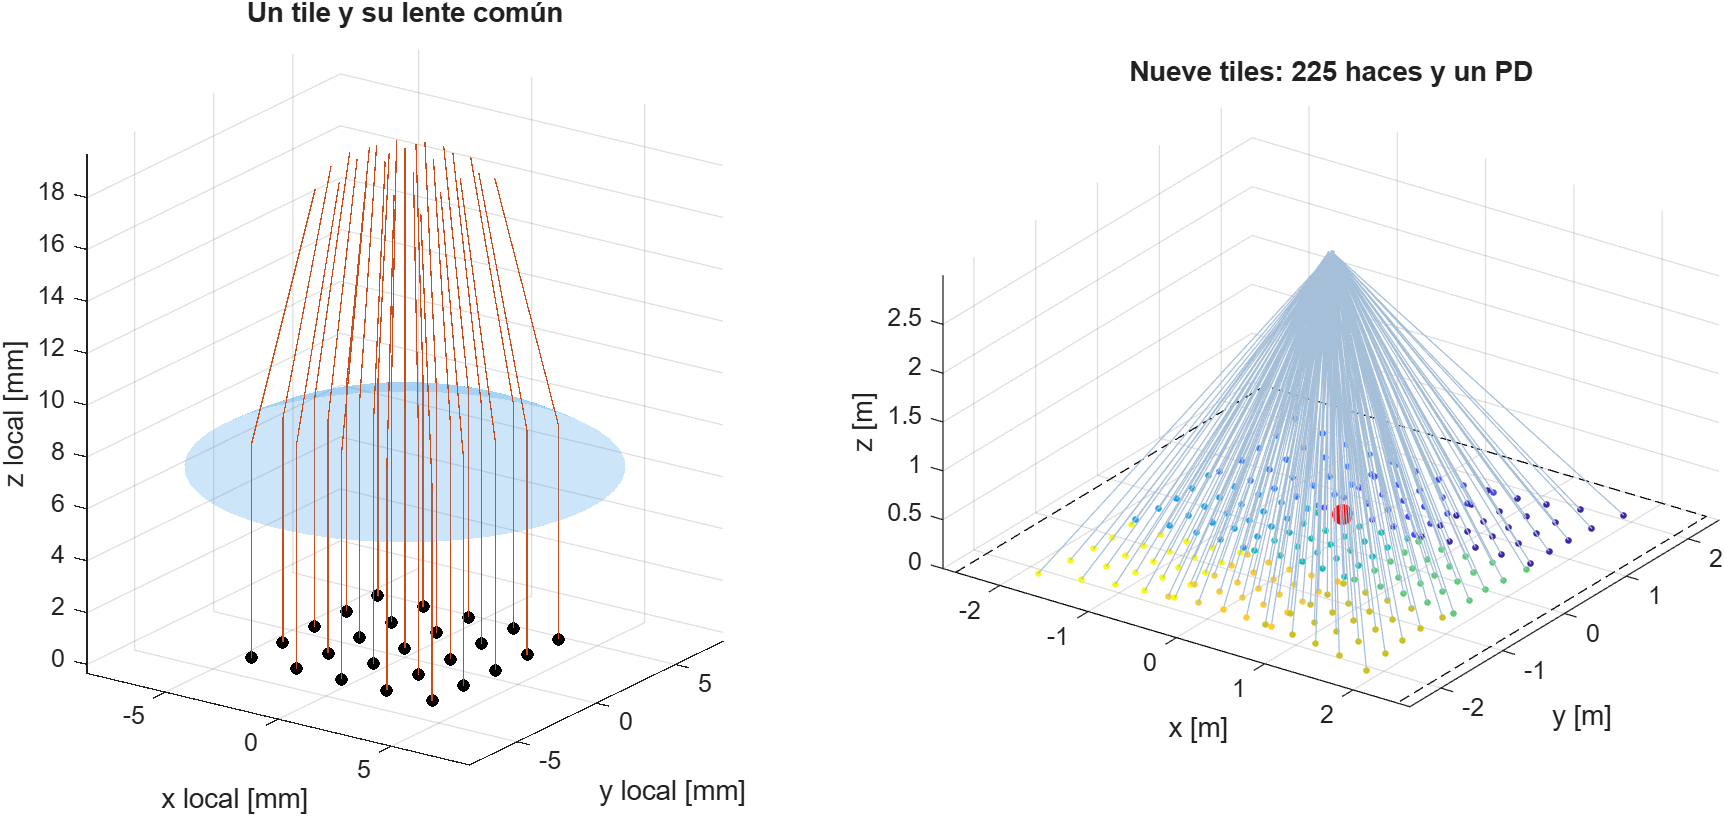
\includegraphics[width=\linewidth]{02_geometria_sistema.png}
\caption{Geometría implementada. Izquierda: un tile y la cara curva común, en escala milimétrica local. Derecha: los 225 ejes del AP y un PD, en coordenadas globales métricas. La primera vista ilustra la óptica, no el tamaño relativo de una habitación.}
\end{figure}

\section{Modelo óptico: de los parámetros a las potencias}
\subsection{Parámetros, hipótesis y convenciones}
\begin{table}[H]\centering
\begin{tabular}{ll}\toprule
Parámetro & Valor inicial\\\midrule
Array por tile y pitch & $5\times5$, $\delta=2$ mm\\
Longitud de onda y waist & $\lambda=950$ nm, $w_0=5\,\mu$m\\
Separación array--cara plana & $d_{VL}=5$ mm\\
Índice, diámetro y curvatura & $n=1.55$, $L=16$ mm, $R=15$ mm\\
Focal efectiva & $f=R/(n-1)=27.2727$ mm\\
Potencia óptica por VCSEL activo & $P_t=10$ mW\\
Espesor de borde supuesto & $t_e=2$ mm\\
Área del único PD y transmisión & $A_{PD}=1$ mm$^2$, $\eta=0.90$\\
Normal y semicampo de visión del PD & $[0,0,1]^T$, $70^\circ$\\
Centro del array central & altura global $H=3$ m\\
AP completo & nueve tiles, separación 20 mm, inclinación $21^\circ$\\\bottomrule
\end{tabular}
\caption{Configuración nominal. $t_e$, el PD único, su FoV, $\eta$ y la electrónica receptora son hipótesis de este estudio, no parámetros inferidos del ADR de Kazemi.}
\end{table}

Las unidades internas son SI. Las posiciones MATLAB son columnas $3\times N$, las potencias son $M\times N$ y los Jacobianos son $M\times3\times N$, con $M=25K$ o $225K$. El orden de canal es estado, tile, VCSEL. El tile central es el número 5 y el VCSEL central el 13, usando índices MATLAB desde uno. Python utilizaba índices 4 y 12; esta diferencia se prueba explícitamente.

Se suponen LoS, VCSELs monomodo TEM$_{00}$ con $M^2=1$, potencia identificable, geometría calibrada y receptor inmóvil durante el barrido. No se incluyen reflexiones, oclusiones, saturación, cuantización ni interferencia de pilotos. Se trabaja con un PD sin CPC, sin concentración y sin diversidad angular receptora. Su área no es una apertura óptica ficticiamente amplificada.

El manuscrito no fija numéricamente el espesor de la lente. Se adopta un borde conocido y se deduce el espesor central por la sagita. Así se define una familia de superficies al variar $R$; no se impone que un actuador comercial cambie su volumen y forma exactamente de ese modo.

\subsection{Posición de emisores y superficie curva}
Se numeran los emisores como $i=5(m-1)+n_c$, para $m,n_c\in\{1,\ldots,5\}$:
\begin{equation}
x_i=(n_c-3)\delta,\qquad y_i=(3-m)\delta,\qquad \rho_i^2=x_i^2+y_i^2.
\end{equation}
El cuadrado entre centros extremos tiene lado 8 mm, distinto de la implantación aproximada de 1 cm$^2$ mencionada en el artículo. Para un estado convexo $R_k>0$:
\begin{align}
t_{c,k}&=t_e+R_k-\sqrt{R_k^2-(L/2)^2},\\
\tau_{i,k}&=\sqrt{R_k^2-\rho_i^2}+t_{c,k}-R_k,\\
\vect o_{i,k}^{loc}&=[x_i,y_i,d_{VL}+\tau_{i,k}]^T.
\end{align}
En el estado inicial se obtiene $t_c=4.3114$ mm. Cada emisor recorre un espesor diferente. El origen posterior a la lente se sitúa en su salida real, no en un origen común aproximado del tile.

\subsection{Demostración de la dirección refractada}
La normal exterior de la superficie convexa es
\begin{equation}
\vect n_{i,k}=\frac{[x_i,y_i,\sqrt{R_k^2-\rho_i^2}]^T}{R_k}.
\end{equation}
Sea $\vect v_1$ unitario, $c=\vect n^T\vect v_1$ y $\mu=n_1/n_2$. Se descompone la dirección en componente normal $c\vect n$ y tangencial $\vect v_1-c\vect n$. Snell multiplica la tangencial por $\mu$. Para que el resultado siga siendo unitario, su componente normal de transmisión debe tener longitud $\sqrt{1-\mu^2(1-c^2)}$. Por tanto,
\begin{equation}\label{eq:snell}
\vect v_2=\mu\vect v_1+
\left[\sqrt{1-\mu^2(1-c^2)}-\mu c\right]\vect n.
\end{equation}
Esto demuestra simultáneamente que la tangencial cumple Snell y que $\|\vect v_2\|=1$, siempre que el discriminante no sea negativo y se elija la rama transmitida.

La incidencia principal sobre la cara plana es normal: no cambia su eje. En la cara curva se toma $\mu=n$, $\vect v_1=\vect e_z$. Reordenando \eqref{eq:snell} se recupera el coeficiente de Kazemi:
\begin{align}
Q_{i,k}&=\frac{\sqrt{R_k^2-n^2\rho_i^2}-n\sqrt{R_k^2-\rho_i^2}}{R_k^2},\\
\vect v_{i,k}^{loc}&=[Q_{i,k}x_i,Q_{i,k}y_i,n+Q_{i,k}\sqrt{R_k^2-\rho_i^2}]^T.
\end{align}
La dependencia de $R_k$ aparece explícitamente en la dirección. No se sustituye esta física por un conjunto de divergencias elegidas arbitrariamente.

Se rechazan superficies imposibles, espesores no positivos, rayos principales fuera de apertura y reflexión interna total del rayo principal. También se calcula una cota de clipping del haz en la apertura. Estas verificaciones no excluyen TIR de las colas; se examina posteriormente mediante ray tracing.

\subsection{Demostración de la transformación del parámetro complejo}
El waist inicial define
\begin{equation}
z_R=\frac{\pi w_0^2}{\lambda},\qquad q_{in}=d_{VL}+jz_R.
\end{equation}
La traslación equivalente dentro del vidrio y la potencia refractiva dan la matriz
\begin{equation}
\begin{bmatrix}A&B\\C&D\end{bmatrix}
=\begin{bmatrix}1&0\\-1/f_k&1\end{bmatrix}
 \begin{bmatrix}1&\tau_{i,k}/n\\0&1\end{bmatrix}
=\begin{bmatrix}1&\tau_{i,k}/n\\-1/f_k&1-\tau_{i,k}/(nf_k)\end{bmatrix},
\qquad f_k=\frac{R_k}{n-1}.
\end{equation}
Su determinante es uno. Aplicando la ley ABCD:
\begin{equation}
q^{out}_{i,k}=\frac{Aq_{in}+B}{Cq_{in}+D}=a_{i,k}+jb_{i,k}.
\end{equation}
Para ver qué se transforma, se define $u=d_{VL}+\tau_{i,k}/n$. Entonces $q^{out}=(u+jz_R)/(1-u/f_k-jz_R/f_k)$. Multiplicar numerador y denominador por el conjugado conduce a
\begin{align}
D_q&=(1-u/f_k)^2+(z_R/f_k)^2,\\
a_{i,k}&=\frac{u(1-u/f_k)-z_R^2/f_k}{D_q},&
b_{i,k}&=\frac{z_R}{D_q}>0.
\end{align}
Tras una distancia axial $s$ desde la salida,
\begin{equation}\label{eq:width}
q_{i,k}(s)=s+a_{i,k}+jb_{i,k},\qquad
W_{i,k}(s)=w_{i,k}^2(s)=\frac{\lambda}{\pi}\frac{(s+a_{i,k})^2+b_{i,k}^2}{b_{i,k}}.
\end{equation}
El waist equivalente está en $\vect o-a\vect v$, su Rayleigh es $b$ y su radio es $\sqrt{\lambda b/\pi}$. No se reinicia artificialmente el waist en la superficie de salida. Las pruebas comprueban las expresiones cerradas, el determinante y el ancho en la salida.

\begin{figure}[H]\centering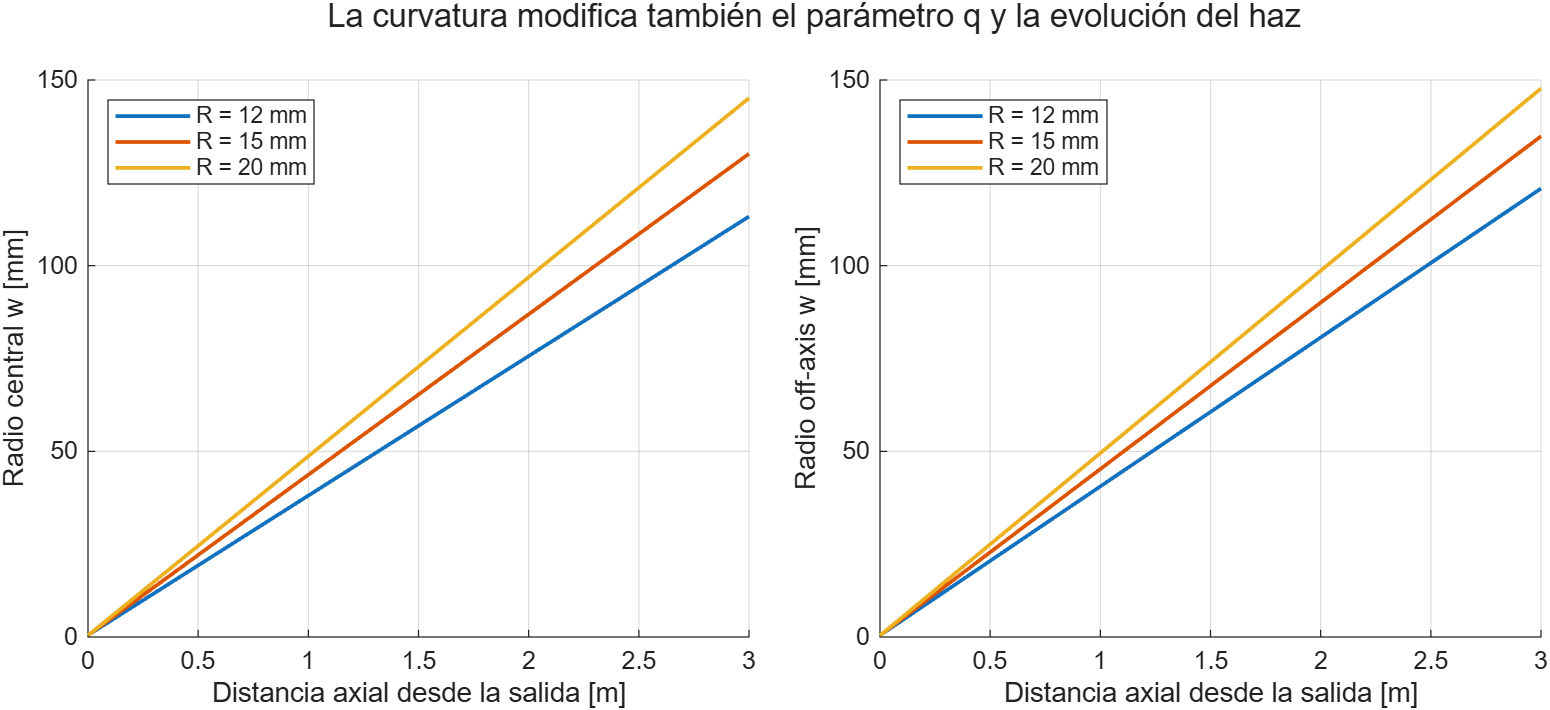
\includegraphics[width=\linewidth]{03_evolucion_gaussian.png}
\caption{La focal modifica el tamaño y la evolución del haz, además de su dirección. El espesor off-axis hace que el mismo estado común no imponga idéntico $q$ a todos los emisores.}
\end{figure}

\subsection{Coordenadas globales y los nueve tiles}
Se aplica a cada tile una rotación
\begin{equation}
\mathcal R_v=R_y(\pi+\beta_v)R_x(\alpha_v),
\quad
\begin{bmatrix}\alpha_v\\\beta_v\end{bmatrix}
=\theta_t\begin{bmatrix}-1&-1&-1&0&0&0&1&1&1\\-1&0&1&1&0&-1&-1&0&1\end{bmatrix}_{:,v}.
\end{equation}
Los desplazamientos de montaje siguen las matrices del artículo. El montaje se mantiene fijo durante el barrido de estados. Las salidas y direcciones se transforman con la misma rotación: $\vect o=\vect r_v+\mathcal R_v\vect o^{loc}$ y $\vect v=\mathcal R_v\vect v^{loc}$.

La expansión escalar de una coordenada en el manuscrito contiene una inconsistencia: el primer componente del término rotado $[0,0,d_c]^T$ es $-d_c\cos\alpha\sin\beta$, no $-d_c\sin\alpha\cos\beta$. Se emplea el producto matricial directamente. También se utilizan las distancias completas entre salidas y PD, no una altura común aproximada en todas las distancias.

El AP completo conserva \textbf{nueve lentes comunes a sus respectivos tiles}, sincronizadas al mismo estado $k$, no una sola lente que abarque los 225 emisores. Esta distinción evita cambiar inadvertidamente la arquitectura al extenderla.

\subsection{De irradiancia a potencia del PD}
Para cada salida y dirección globales,
\begin{equation}
\vect d=\vect p-\vect o,\quad s=\vect v^T\vect d,\quad
\vect t=\vect d-s\vect v,\quad r^2=\|\vect t\|^2.
\end{equation}
El perfil Gaussian es $I=2P_t\exp(-2r^2/W)/(\pi W)$. Su normalización se verifica analíticamente:
\begin{equation}
\int_0^\infty\frac{2P_t}{\pi W}e^{-2r^2/W}2\pi r\,dr=P_t,
\end{equation}
pues el cambio $u=2r^2/W$ reduce la integral a $P_t\int_0^\infty e^{-u}du$.

Con un PD pequeño respecto de la mancha,
\begin{equation}\label{eq:power}
P_{i,k}(\vect p)=\frac{2P_t\eta A_{PD}}{\pi W_{i,k}(s)}
 e^{-2r^2/W_{i,k}(s)}\max(0,-\vect n_{PD}^T\vect v_{i,k})
 \mathbf 1_{FoV}\mathbf 1_{s>0}.
\end{equation}
La unidad es W: irradiancia W/m$^2$ por área m$^2$. El signo menos es necesario porque $\vect v$ apunta hacia el receptor y la normal del PD hacia el techo. Con esas convenciones, usar el signo positivo daría incidencia inválida incluso al haz central.

Se conserva la aproximación del artículo de utilizar el eje del haz para la incidencia. La dirección local del flujo de un frente curvo puede diferir de él. Tampoco se modela aquí la astigmatización mediante dos parámetros $q$ distintos. Las validaciones posteriores delimitan estas aproximaciones. Una prueba integra sobre un cuadrado receptor de $1\times1$ mm$^2$ y contrasta el modelo puntual en un punto representativo.

\subsection{Extensión exploratoria de curvatura negativa}
Para estudiar si un mayor solapamiento ayuda, se permite una superficie plano-cóncava con $R<0$. No se obtiene cambiando solamente el signo de una divergencia:
\begin{align}
t_c&=t_e+\operatorname{sign}(R)\left(|R|-\sqrt{R^2-(L/2)^2}\right),\\
\tau_i&=t_c+\operatorname{sign}(R)\left(\sqrt{R^2-\rho_i^2}-|R|\right),\\
\vect n_i&=[x_i/R,y_i/R,\sqrt{1-\rho_i^2/R^2}]^T.
\end{align}
Se vuelve a aplicar Snell y la transformación ABCD con focal negativa. Los estados exploratorios usan borde de 6 mm para mantener espesor positivo. Es una modificación adicional del diseño de Kazemi, cuya validez se debe comprobar; sus resultados Gaussian favorables no bastan para recomendar hardware.

\textbf{Archivos del capítulo:} \archivo{configuracion/gob_config.m}, \archivo{modelo/gob_model.m}, \archivo{modelo/gob_rotation.m}, \archivo{modelo/gob_power.m}, \archivo{modelo/gob_diagnostics.m} y \archivo{pruebas/test_gob_model.m}.

\section{Identificabilidad: demostraciones y límites}
\subsection{Una explicación analítica del caso 2D}
\begin{proposicion}[Modelo simplificado de manchas de igual ancho]
En un plano conocido, supóngase $P_i(\vect x)=c_i\exp(-2\|\vect x-\vect b_i\|^2/w^2)$, con $c_i>0$, ancho común conocido y centros conocidos. Si dos diferencias de centros respecto de un emisor de referencia son linealmente independientes, las razones de esas tres potencias determinan de forma única $\vect x=[x,y]^T$ dentro de este modelo.
\end{proposicion}
\begin{proof}
Al tomar el logaritmo de una razón se elimina cualquier escala común:
\begin{align}
\log(P_i/P_j)-\log(c_i/c_j)
&=-\frac2{w^2}\bigl(\|\vect x-\vect b_i\|^2-\|\vect x-\vect b_j\|^2\bigr)\\
&=\frac4{w^2}(\vect b_i-\vect b_j)^T\vect x
-\frac2{w^2}(\|\vect b_i\|^2-\|\vect b_j\|^2).
\end{align}
Dos razones proporcionan un sistema lineal $2\times2$. La hipótesis de independencia equivale a determinante no nulo; por tanto el sistema tiene una única solución.
\end{proof}

Esta proposición explica de dónde proviene la diversidad espacial, pero \textbf{no demuestra inyectividad global del modelo completo} con anchos off-axis diferentes, distancias axiales variables y máscaras. Tampoco legitima tomar logaritmos de señales débiles o negativas. El estimador real utiliza potencias lineales con ruido; la demostración es una herramienta de interpretación.

El etiquetado es importante: reflejar una posición en un array simétrico suele permutar los canales. El vector etiquetado cambia, aunque la suma de potencias pueda ser igual. La prueba \archivo{testLabelSymmetry} verifica precisamente igual suma y vectores distintos. No se infiere unicidad de la potencia total.

\subsection{Por qué una focal puede bastar para 3D calibrado}
En campo lejano y para una dirección fija $\vect u$, el modelo tiene la estructura aproximada
\begin{equation}\label{eq:farfield}
\vect P(d,\vect u)\simeq d^{-2}\vect a(\vect u),
\end{equation}
donde $d$ es la distancia al origen óptico de referencia y $\vect a$ incorpora direcciones, divergencias y factores de incidencia. Las razones entre canales dependen sobre todo de $\vect u$; una vez determinada la dirección, un canal no nulo permite recuperar la escala:
\begin{equation}
d\simeq\sqrt{a_i(\vect u)/P_i},\qquad \vect p\simeq\vect p_{AP}+d\vect u.
\end{equation}
No es una triangulación con grandes distancias entre emisores: es una combinación de información angular y \emph{rango radiométrico}. La potencia, transmisión, área efectiva y ganancia electrónica deben estar calibradas. Este mecanismo ya existe con $K=1$.

\subsection{Demostración de la ambigüedad con ganancia libre}
\begin{proposicion}[Invariancia de campo lejano]
Si la observación de uno o varios estados es $\vect y=(g/d^2)\vect a(\vect u)$ con $g>0$ desconocido, no pueden determinarse simultáneamente $d$ y $g$ a partir de esa observación.
\end{proposicion}
\begin{proof}
Para cualquier $c>0$, tomar $d'=cd$ y $g'=c^2g$ deja $g'/d'^2=g/d^2$. Hay una familia continua de pares distintos con idéntica observación. Concatenar varios estados solo reemplaza $\vect a$ por $[\vect a_1^T,\ldots,\vect a_K^T]^T$, sin eliminar la invariancia.

La misma degeneración aparece en el Jacobiano: $\partial\vect y/\partial d=-2\vect y/d$ y $\partial\vect y/\partial\log g=\vect y$. Ambas columnas son proporcionales. Una vez eliminada la ganancia como parámetro nuisance, no queda información radial en este modelo límite.
\end{proof}

El modelo geométrico completo no es exactamente \eqref{eq:farfield}: las salidas y los waists están separados, y los nueve tiles añaden pequeños desplazamientos. Estas correcciones pueden dar rango formal completo y mejorar algunos puntos. No se afirma imposibilidad absoluta para cualquier SNR. Lo que se comprueba es que, a la escala métrica ensayada, esa información puede ser demasiado débil y sensible a calibración para una altura robusta.

Una incertidumbre de escala produce, linealizando $d\propto\sqrt{g}$,
\begin{equation}
\frac{\Delta d}{d}\simeq\frac12\frac{\Delta g}{g}.
\end{equation}
A 3 m, 1\% de error de ganancia puede corresponder a unos 15 mm de error radial. Esta sensibilidad explica por qué el caso calibrado no representa el caso de ganancia desconocida.

\begin{figure}[H]\centering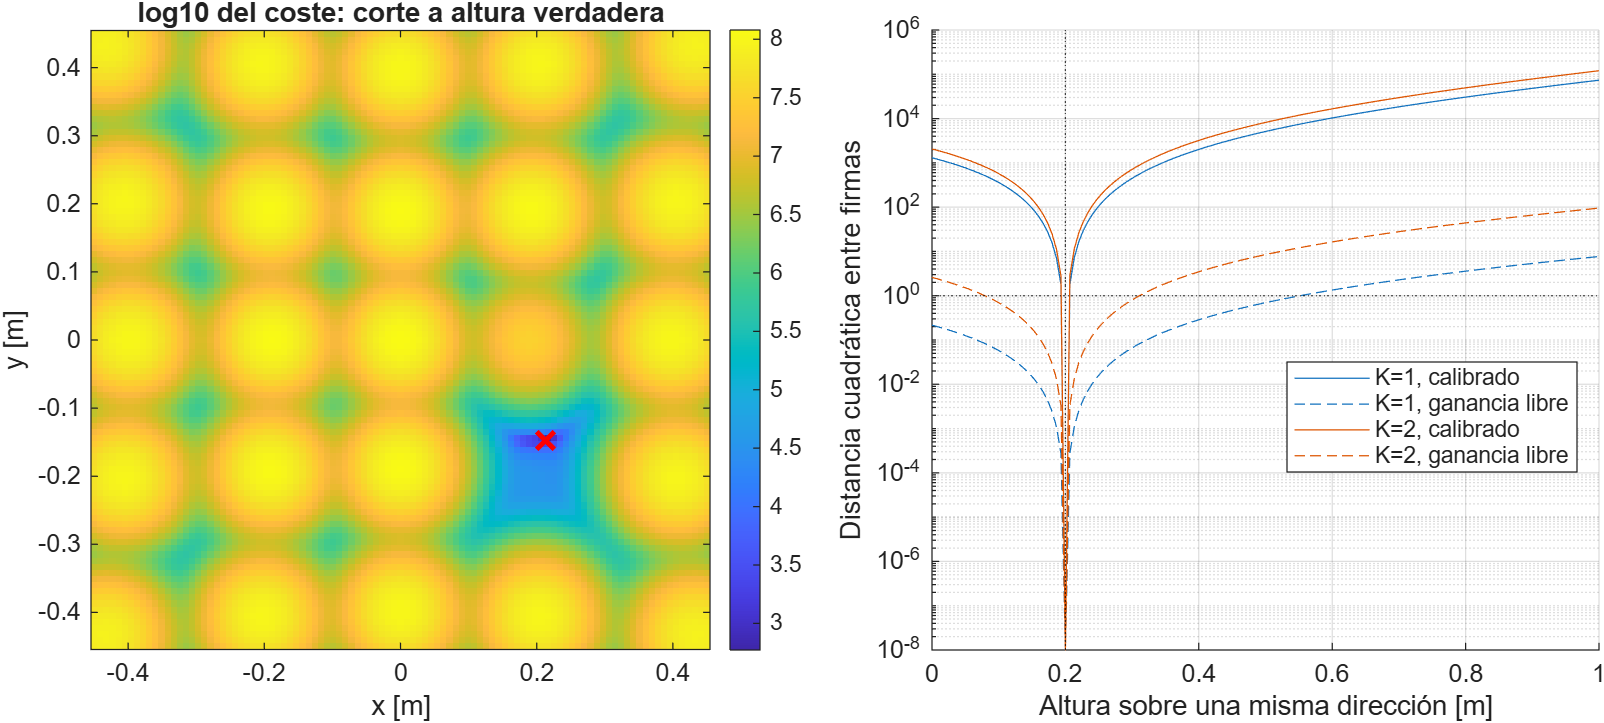
\includegraphics[width=\linewidth]{04_coste_y_ambiguedad.png}
\caption{Izquierda: corte del coste a altura verdadera, usado solo para visualizar, no para inicializar el estimador 3D. La cruz marca la verdad; la malla de 9 mm no incluye necesariamente ese mínimo de coste cero. Derecha: comparación de firmas sobre una misma dirección espacial; perfilar la ganancia reduce notablemente la discriminación de altura. La horizontal uno corresponde a distancia cuadrática de una unidad de ruido.}
\end{figure}

\subsection{Demostración del Jacobiano completo}
Se escribe $W=w^2$, $s=\vect v^T\vect d$ y $\vect t=(I-\vect v\vect v^T)\vect d$. Al ser $\vect v$ unitario y fijo en un estado,
\begin{equation}
\nabla s=\vect v,\qquad \nabla r^2=2\vect t,\qquad
\nabla W=\frac{2\lambda}{\pi b}(s+a)\vect v.
\end{equation}
Dentro de una región visible regular, los factores de incidencia del modelo de eje no dependen de la posición. Por tanto,
\begin{align}
\log P&=\log C-\log W-2r^2/W,\\
\nabla\log P&=-\frac{\nabla W}{W}-\frac{2\nabla r^2}{W}+\frac{2r^2\nabla W}{W^2},\\
\boxed{\nabla P=P\left[\left(\frac{2r^2}{W^2}-\frac1W\right)\nabla W-\frac{4\vect t}{W}\right].}
\end{align}
La implementación usa esta expresión y la contrasta con diferencias centradas de paso $10^{-6}$ m. Se prueban uno y nueve tiles, varios estados, esquinas y casos cóncavos. El Jacobiano no se deduce ajustando datos de prueba.

\subsection{Rango local no equivale a unicidad global}
\begin{proposicion}[Condición suficiente local]
Sea $\vect y:\mathcal U\subset\R^d\to\R^M$ diferenciable, $d=2$ o 3. Si su Jacobiano tiene rango columna $d$ en $\vect p_0$, existe un entorno de $\vect p_0$ donde el mapa es inyectivo.
\end{proposicion}
\begin{proof}
Existe un menor $d\times d$ no singular. Seleccionando esas $d$ observaciones se obtiene un submapa cuyo Jacobiano cuadrado es invertible. El teorema de la función inversa da una inversa local de ese submapa. Si dos puntos próximos tuviesen la misma observación completa, tendrían también el mismo subvector y serían el mismo punto.
\end{proof}

La conclusión es local. Dos puntos lejanos podrían tener firmas iguales o casi iguales; además, un menor puede ser no nulo pero numéricamente minúsculo. Por eso se estudian singularidades ponderadas por ruido, mínimos alternativos, recuperación sin ruido y errores con ruido. Una malla finita no demuestra inyectividad en todo un volumen continuo.

\subsection{Información de posición y ganancia nuisance}
Con $J=\partial\vect P/\partial\vect p$ y covarianza fija positiva $\Sigma$,
\begin{equation}
J_w=\Sigma^{-1/2}J,\quad F_\mu=J_w^T J_w,\quad
\operatorname{PEB}_\mu=\sqrt{\operatorname{tr}(F_\mu^{-1})}.
\end{equation}
Si $J_w=U\operatorname{diag}(s_1,\ldots,s_d)V^T$, entonces
\begin{equation}
F_\mu^{-1}=V\operatorname{diag}(s_1^{-2},\ldots,s_d^{-2})V^T.
\end{equation}
Esta expresión explica la implementación por SVD y la dominancia del menor valor singular. Si falta rango se devuelve $\infty$, no una pseudoinversa que elimine la dirección no observable. Se utilizan umbrales $s_d>10^{-9}s_1$ y $s_d>10^{-12}$ en el Jacobiano ponderado.

Si $G_w$ contiene las derivadas ponderadas respecto de parámetros nuisance de ganancia, el complemento de Schur es
\begin{equation}
F_{p|g}=J_w^T\left[I-G_w(G_w^TG_w)^{-1}G_w^T\right]J_w.
\end{equation}
La matriz entre corchetes es la proyección ortogonal fuera del espacio generado por la ganancia. Es semidefinida positiva y no mayor que $I$; introducir una ganancia desconocida nunca aumenta la información de posición. Se comprueba con una ganancia común y con una por estado. El código trata columnas nulas sin invertir una norma cero.

\textbf{Matiz estadístico importante.} El ruido utilizado depende ligeramente de la potencia. La información exacta de un modelo Gaussian heteroscedástico incluiría también
\begin{equation}
[F_{\Sigma}]_{ab}=\tfrac12\operatorname{tr}(\Sigma^{-1}\Sigma_{,a}\Sigma^{-1}\Sigma_{,b}).
\end{equation}
Aquí se publica la información de la media con covarianza congelada, no se explota ese segundo término como sensor de posición. Por ello $\operatorname{PEB}_\mu$ es una medida local del modelo de media/covarianza fijada; \textbf{no debe denominarse CRLB exacta del modelo heteroscedástico completo}. Tampoco garantiza errores de un estimador sesgado o sujeto a fronteras. Un estimador acotado en una caja puede tener error inferior a una cota local enorme sin contradicción: se han perdido las hipótesis de insesgadez y regularidad de esa cota.

\textbf{Archivos del capítulo:} \archivo{modelo/gob_power.m}, \archivo{estimacion/gob_information.m}, \archivo{experimentos/gob_controls.m}, \archivo{pruebas/test_gob_inference.m} y \archivo{pruebas/test_gob_reference.m}.

\section{Ruido, adquisición y algoritmo de estimación}
\subsection{Modelo de ruido en unidades de potencia}
La medida simulada es $y_\ell=P_\ell(\vect p)+\varepsilon_\ell$, con ruido Gaussian independiente por piloto y desviación
\begin{equation}\label{eq:noise}
\sigma_P^2(P)=\frac{B}{\mathcal R^2}\left[
\frac{4k_BT}{R_f}+i_a^2+2q_e(\mathcal RP+I_{bg})+
\mathrm{RIN}(\mathcal RP)^2\right]+(\epsilon P)^2.
\end{equation}
La responsividad $\mathcal R$ convierte potencia en corriente; los términos entre corchetes son densidades espectrales de corriente, que se integran sobre el ancho de banda $B$ y se vuelven a expresar en W$^2$. Se incluyen ruido térmico, amplificador, shot de señal y fondo, RIN y una fluctuación multiplicativa por piloto.

\begin{table}[H]\centering\begin{tabular}{ll}\toprule
Parámetro & Valor\\\midrule
$\mathcal R$ & 0.7 A/W\\
$T$, $R_f$ & 300 K, 10 k$\Omega$\\
$i_a$ & 2 pA/$\sqrt{\mathrm{Hz}}$\\
$I_{bg}$, con media sustraída & 10 $\mu$A\\
RIN & $-155$ dB/Hz\\
$\epsilon$ & 0.5\%, independiente entre pilotos\\
$B_0$ de referencia & 100 Hz\\
Desviación sin señal, $B=B_0$ & aproximadamente 42.53 pW\\\bottomrule
\end{tabular}\caption{Hipótesis de electrónica para el PD único. No se utiliza el ancho de banda de 2 GHz del receptor de comunicaciones del artículo.}\end{table}

La componente multiplicativa no representa un error fijo de calibración: es una fluctuación independiente entre adquisiciones. Las incertidumbres persistentes por VCSEL, focal o ganancia común se tratan como perturbaciones separadas. No deben confundirse porque promediar puede reducir la primera, pero no corregir las segundas.

\subsection{Comparación justa del número de estados}
Se usa encendido secuencial, de modo que el shot de señal corresponde al emisor activo. Para una integración rectangular de duración $T_{int}$, la banda equivalente unilateral es $B=1/(2T_{int})$. Se fija
\begin{equation}
B_K=100K\ \mathrm{Hz},\qquad T_{int,K}=\frac1{200K}\ \mathrm{s}.
\end{equation}
El tiempo de integración de $25K$ pilotos es 125 ms por tile; para $225K$, 1.125 s. Así, aumentar $K$ no recibe gratuitamente más tiempo de integración.

Esta igualdad no incluye asentamiento de la lente ni procesamiento. Tampoco hace equivalente un sistema de pilotos simultáneos: encender varios emisores cambia shot, RIN e interferencia. La posible reducción de latencia mediante pilotos ortogonales requiere un modelo de adquisición distinto. Las simulaciones presuponen posición constante durante todo el barrido.

Se incluye un control especialmente importante: repetir exactamente $R=15$ mm dos y ocho veces. Ese control puede promediar la fluctuación multiplicativa independiente, pero no aporta nueva geometría. Compararlo con estados distintos permite separar promediado y diversidad real.

\subsection{Función objetivo sin información de la posición verdadera}
El generador conoce la verdad para crear datos; el estimador no la recibe. Sus pesos se calculan con las medidas:
\begin{equation}
\widehat\sigma_\ell=\sigma_P(\max(y_\ell,0)),\qquad
\widehat{\vect p}=\arg\min_{\vect p\in\mathcal B}
\sum_\ell\frac{(P_\ell(\vect p)-y_\ell)^2}{\widehat\sigma_\ell^2}.
\end{equation}
Esto es mínimos cuadrados ponderados factibles, no máxima verosimilitud exacta del modelo heteroscedástico. Las medidas negativas después de sustraer fondo se conservan en el residuo. Solo se limitan a cero al evaluar la varianza y la firma comprimida de inicialización.

Si la ganancia es desconocida, el estado es $[x,y,z,\gamma]^T$, con $g=e^\gamma$, y el residuo es $(gP-y)/\widehat\sigma$. Se usan límites $0.2\le g\le5$. Para altura conocida se omite $z$ del estado. La derivada adicional respecto de $\gamma$ es $gP$, y la de posición es $gJ$.

\subsection{Biblioteca, varios arranques y ajuste local}
El procedimiento implementado es:
\begin{enumerate}
\item Construir una biblioteca de potencias del modelo en una malla de la caja de búsqueda.
\item Ordenar los candidatos por coste ponderado. Si la ganancia es libre, perfilar su valor inicial mediante $g=\langle P,y\rangle_w/\langle P,P\rangle_w$, limitado al intervalo admisible.
\item Ordenar también por distancia entre firmas $\operatorname{asinh}(P/\sigma_{oscuro})$. Esta compresión evita que un ligero desajuste de malla de un canal fuerte descarte la región correcta.
\item Intercalar ambos órdenes y seleccionar seis semillas separadas al menos 12 cm.
\item Ejecutar \archivo{lsqnonlin}, con Jacobiano analítico, restricciones de caja y algoritmo trust-region-reflective.
\item Conservar la solución de menor coste y registrar mínimos alternativos separados más de 10 cm.
\end{enumerate}
La compresión \emph{no} cambia el modelo de observación ni el ajuste final: únicamente elige candidatos. La malla de inicialización es distinta de las posiciones aleatorias y de la malla de evaluación. Para el estudio se utilizan $35\times35$ candidatos laterales por tile, $51\times51$ para nueve tiles y nueve alturas en 3D. Las variables internas del optimizador y las semillas quedan accesibles en el struct devuelto.

No se promete encontrar el mínimo global de una función no convexa. La convergencia de \archivo{lsqnonlin} se informa por separado del error real en simulación. En un punto oscuro, un algoritmo puede converger y seguir siendo incapaz de proporcionar una localización útil.

\subsection{Regresión que comprueba la búsqueda}
En Python se encontró una observación del AP completo cuya posición verdadera era aproximadamente $(-0.1024,-1.0424,0)$ m. La búsqueda basada solo en coste ponderado arrancaba en una región errónea y terminaba a 1.396 m de la verdad, pese a una información local favorable. Se introdujo la búsqueda combinada, sin suministrar la verdad al algoritmo.

La observación concreta se conserva como referencia y se vuelve a ajustar en MATLAB. \archivo{testOriginalInitializerRegression} exige error inferior a 1 mm y coste inferior a 600. Se verifica así el mecanismo que resolvió el fallo, no solo que MATLAB ejecuta la sintaxis.

\textbf{Archivos del capítulo:} \archivo{configuracion/gob_noise.m}, \archivo{modelo/gob_sigma.m}, \archivo{estimacion/gob_estimator.m}, \archivo{estimacion/gob_candidate_costs.m}, \archivo{estimacion/gob_residual.m}, \archivo{estimacion/gob_fit.m} y \archivo{demo_localizacion.m}.

\section{Diseño de experimentos y trazabilidad de las pruebas}
\subsection{Regiones: no confundir un núcleo útil con un noveno nominal}
Para un semiancho $a$ en el plano de referencia se define
\begin{equation}\label{eq:domain}
\mathcal V_a=\{(x,y,z):0\le z\le1,\ |x|,|y|\le a(3-z)/3\}.
\end{equation}
Es un tronco de pirámide, no un prisma. La sección se contrae con la altura porque una huella angular cubre menos superficie cerca del techo. Se ensayan también prismas $|x|,|y|\le a$, $0\le z\le1$, para no extrapolar injustificadamente resultados a esquinas superiores no iluminadas.

\begin{table}[H]\centering\begin{tabular}{lll}\toprule
$a$ & Base en $z=0$ & Interpretación\\\midrule
0.45 m & $0.90\times0.90$ m$^2$ & Núcleo de un tile\\
0.60 m & $1.20\times1.20$ m$^2$ & Núcleo ampliado\\
$5/6$ m & $1.667\times1.667$ m$^2$ & Noveno nominal de 25 m$^2$\\
1.80 m & $3.60\times3.60$ m$^2$ & Región central del AP completo\\
2.50 m & $5.00\times5.00$ m$^2$ & Huella nominal completa\\\bottomrule
\end{tabular}\caption{La sección en $z=1$ tiene $2/3$ del lado de la base. El receptor 3D no se restringe a una altura conocida.}\end{table}

La caja de búsqueda del estimador es la envolvente rectangular de la región. No se le da la relación del borde \eqref{eq:domain} como una ecuación para determinar la altura. Tampoco se le indica el tile dominante correcto.

\subsection{Demostración del muestreo uniforme en volumen}
Una altura uniforme no produciría densidad uniforme en un tronco cuya sección cambia. El área de sección es $A(z)=4a^2(3-z)^2/9$. El volumen es
\begin{equation}
V_a=\int_0^1 A(z)\,dz=4a^2\frac{19}{27}.
\end{equation}
Para densidad espacial constante, la función acumulada de altura debe ser
\begin{equation}
F_z(z)=\frac{\int_0^z A(t)dt}{V_a}=\frac{27-(3-z)^3}{19}.
\end{equation}
Por inversión, con $U\sim\mathcal U(0,1)$:
\begin{equation}
z=3-(27-19U)^{1/3}.
\end{equation}
Condicionadas a esa altura, $x$ e $y$ se sortean uniformemente en su sección. El código implementa exactamente esta construcción. Para el prisma se usan las tres coordenadas uniformes en sus intervalos.

\subsection{Tamaño, semillas y estadísticas}
Cada caso principal tiene 300 posiciones aleatorias. Se añaden nueve puntos estructurados en 2D y 27 en 3D: combinaciones de coordenadas extremas y centrales en las alturas 0, 0.5 y 1 m. Los errores de estos puntos no se mezclan con los percentiles aleatorios; se informan por separado.

Los mapas finales utilizan $61\times61$ puntos en 2D y $61\times61\times5$ en 3D. El barrido de diseño utiliza una malla distinta, generalmente $17\times17\times5$; el barrido de inclinación usa $25\times25\times5$. La fracción de puntos de una malla no equivale a una fracción volumétrica, mientras que Monte Carlo sí sigue el volumen definido.

El generador MATLAB es \archivo{mt19937ar}, con semilla 20260912 para el estudio; 20260912+9000 para auditorías sin ruido y 20260912+3000 para sensibilidad. El ray tracing usa semilla 193 y muestras antitéticas. Python utilizaba PCG64, por lo que el mismo entero de semilla no genera las mismas posiciones. Se emplean nuevas realizaciones MATLAB y se identifica explícitamente esa diferencia.

El percentil de errores utiliza interpolación lineal con índice $1+(N-1)p$, equivalente a la convención de NumPy utilizada antes. Para mapas que contienen $\infty$ se usa el estadístico ordenado inferior, evitando operaciones indefinidas entre infinitos. No se eliminan los puntos no observables para mejorar artificialmente un promedio.

Para una tasa observada de fallo $\hat p$ y $N$ ensayos, se utiliza el intervalo de Wilson, con $z_{.975}=1.95996$:
\begin{equation}
\frac{\hat p+z_{.975}^2/(2N)\ \pm\ z_{.975}\sqrt{\hat p(1-\hat p)/N+z_{.975}^2/(4N^2)}}{1+z_{.975}^2/N}.
\end{equation}
Con cero fallos en 300 realizaciones, el extremo superior sigue siendo aproximadamente 1.26\%. Por tanto, ``300/300 por debajo de 10 cm'' no es una garantía de fallo nulo.

\subsection{Catálogo de los 25 casos principales}
Los identificadores C01--C25 del resto de las tablas corresponden al catálogo siguiente. La columna de dominio indica tronco (T) o prisma (P); las variantes con ganancia libre son parámetros nuisance, no una calibración de ganancia conocida.
\begingroup\small\setlength{\tabcolsep}{3pt}
\begin{longtable}{lp{7.0cm}rrlp{2.5cm}}\toprule
ID & Nombre del caso & Dim. & Base [m] & Dom. & $R$ [mm]\\\midrule\endhead
C01 & \path{tile_baseline_core_2d} & 2 & 0.9 & T & 15 \\
C02 & \path{tile_baseline_core_3d} & 3 & 0.9 & T & 15 \\
C03 & \path{tile_baseline_ninth_2d} & 2 & 1.67 & T & 15 \\
C04 & \path{tile_baseline_ninth_3d} & 3 & 1.67 & T & 15 \\
C05 & \path{tile_convex_core_2d} & 2 & 1.2 & T & 12, 15 \\
C06 & \path{tile_convex_core_3d} & 3 & 1.2 & T & 12, 15 \\
C07 & \path{tile_diverging_ninth_2d} & 2 & 1.67 & T & -10, -11 \\
C08 & \path{tile_diverging_ninth_3d} & 3 & 1.67 & T & -10, -11 \\
C09 & \path{grid_baseline_full_2d} & 2 & 5 & T & 15 \\
C10 & \path{grid_baseline_full_3d} & 3 & 5 & T & 15 \\
C11 & \path{grid_convex_core_2d} & 2 & 3.6 & T & 12, 15 \\
C12 & \path{grid_convex_core_3d} & 3 & 3.6 & T & 12, 15 \\
C13 & \path{grid_diverging_full_2d} & 2 & 5 & T & -10, -11 \\
C14 & \path{grid_diverging_full_3d} & 3 & 5 & T & -10, -11 \\
C15 & \path{grid_convex_retilted_full_2d} & 2 & 5 & T & 10, 12, 15 \\
C16 & \path{grid_convex_retilted_full_3d} & 3 & 5 & T & 10, 12, 15 \\
C17 & \path{tile_convex_ninth_3d} & 3 & 1.67 & T & 12, 15 \\
C18 & \path{tile_scan8_ninth_3d} & 3 & 1.67 & T & 10, 11, 12, 13, 15, 17, 20, 25 \\
C19 & \path{tile_diverging_single_3d} & 3 & 1.67 & T & -10 \\
C20 & \path{grid_convex_full_3d} & 3 & 5 & T & 12, 15 \\
C21 & \path{tile_diverging_prism_3d} & 3 & 1.67 & P & -10, -11 \\
C22 & \path{grid_diverging_prism_3d} & 3 & 5 & P & -10, -11 \\
C23 & \path{tile_baseline_core_3d_unknown_gain} & 3 & 0.9 & T & 15 \\
C24 & \path{tile_diverging_ninth_3d_unknown_gain} & 3 & 1.67 & T & -10, -11 \\
C25 & \path{grid_diverging_full_3d_unknown_gain} & 3 & 5 & T & -10, -11 \\
\bottomrule\end{longtable}\endgroup


La progresión no se ha limitado a seleccionar casos favorables:
\begin{itemize}
\item \textbf{Una focal convexa:} $R=15$ mm, primero núcleo y después noveno nominal.
\item \textbf{Dos focales convexas:} $R=12,15$ mm para ampliar la región; se prueban también regiones nominales y fronteras.
\item \textbf{Ocho estados:} $R=10,11,12,13,15,17,20,25$ mm para comprobar si muchos estados reparan los huecos.
\item \textbf{Familia cóncava exploratoria:} $R=-10,-11$ mm y borde 6 mm, sin cambiar los VCSELs ni el pitch.
\item \textbf{Nueve tiles:} geometría original de $21^\circ$, núcleo, huella nominal y prisma. También se prueba $27^\circ$ y tres estados $R=10,12,15$ mm.
\item \textbf{Ganancia común desconocida:} núcleo de un tile, tile cóncavo y AP cóncavo completo, con ganancia verdadera 1.08. Sus mapas de información se normalizan a ganancia uno para comparar geometría; sus ensayos estiman la ganancia real.
\end{itemize}

\subsection{Barridos y controles que acompañan a Monte Carlo}
\begin{longtable}{p{4.5cm}p{10cm}}\toprule
Tabla en \archivo{tablas/} & Pregunta que responde\\\midrule\endhead
\archivo{design_sweep.csv} & Pitch 1.5, 2, 2.25 y 2.5 mm; estados individuales, pares y barridos amplios. También separación array--lente de 1 mm, waists 3 y 2 $\mu$m y array mayor de pitch 4 mm/lente 28 mm. Las configuraciones se guardan además en MAT.\\
\archivo{design_rejected.csv} & Geometrías individuales rechazadas por restricciones de lente; no son fallos ocultados de localización.\\
\archivo{diversity_controls.csv} & Repetir el mismo estado frente a variar R; ganancia conocida, común libre y por estado.\\
\archivo{grid_tilt_sweep.csv} & Inclinaciones 21, 24, 27, 30 y 33 grados y seis conjuntos de estados.\\
\archivo{noise_area_tradeoff.csv} & Banda de referencia 10--10000 Hz y áreas de PD 0.1, 1 y 10 mm$^2$. La electrónica y el fondo se mantienen fijos: no es una optimización de capacitancia real.\\
\archivo{radial_ambiguity.csv} & Comparación de dos posiciones separadas aproximadamente 0.60 m sobre una misma dirección, con y sin ajuste de ganancia.\\
\archivo{robustness.csv} & Ocho condiciones en cuatro configuraciones, 100 posiciones por condición: 3200 ajustes.\\
\archivo{ray_validation.csv} & Quince combinaciones de curvatura y emisor, 200000 rayos cada una.\\\bottomrule
\end{longtable}

\subsection{Perturbaciones de calibración}
La sensibilidad se estudia sin informar al estimador de las perturbaciones: control concordante, +2\% de ganancia, 1\% de error fijo por VCSEL compartido entre estados, fondo residual 0.1 nW, PD inclinado $3^\circ$, errores de R de 0.1\% y 1\%, y borde aumentado 0.1 mm. Se comparten realizaciones de ruido entre condiciones para comparar cambios controlados. Se conservan verdad, medias, medidas y estimaciones, no únicamente una tabla final.

\subsection{Trazado de rayos independiente}
El generador de rayos parte del waist con desviaciones de posición $w_0/2$ y pendientes $\lambda/(2\pi w_0)$. Traza la cara plana, intersección exacta con la esfera y refracción de salida por \eqref{eq:snell}. Descarta rayos fuera de apertura, TIR y propagación inversa. Después calcula centroide, matriz de covarianza transversal y radios $2\sqrt{\lambda_j(C)}$.

La referencia circular sobre un plano inclinado tiene covarianza aproximada
\begin{equation}
C_{xy}^{ABCD}=\frac{w^2}{4}\left[I_2+\frac{\vect v_{xy}\vect v_{xy}^T}{v_z^2}\right].
\end{equation}
Comparar ambas covarianzas distingue la elipse de proyección geométrica de la astigmatización que el $q$ circular no recoge. El momento cuarto de Mahalanobis se divide por ocho, su valor esperado para un Gaussian bidimensional ideal.

Se prueban $R=12,15,-10,-11,10$ mm en emisor central 13, lateral 3 y esquina 1: tres millones de rayos. Es una comprobación geométrica, no una simulación electromagnética coherente, una réplica certificada de Zemax ni una prueba de laboratorio. No incluye Fresnel angular ni rugosidad. Su finalidad es detectar cuándo no debe confiarse en la precisión del modelo circular.

\textbf{Archivos del capítulo:} \archivo{configuracion/gob_study_cases.m}, \archivo{configuracion/gob_run_options.m}, las funciones de \archivo{experimentos/}, \archivo{validacion/gob_trace_beam.m} y \archivo{modelo/gob_snell.m}.

\section{Resultados MATLAB, interpretación y decisión}
\subsection{Primero: la solución más simple que funciona}
La ejecución principal corresponde a \DirectorioResultados. Las cifras que siguen se generan leyendo los datos MATLAB de esa ejecución, no transcribiendo los resultados Python.

\begin{table}[H]\centering
\begin{tabular}{lrrrr}\toprule
Arquitectura & $K$ & Lado base [m] & P95 2D [mm] & P95 3D [mm]\\\midrule
Un tile mínimo & 1 & 0.9 & 1.31 & 11.7 \\
Un tile ampliado & 2 & 1.2 & 1.11 & 12 \\
Nueve tiles, $21^\circ$ & 2 & 3.6 & 1.12 & 11 \\
\bottomrule\end{tabular}

\caption{Percentil 95 del error euclídeo en realizaciones aleatorias. El lado corresponde a la base cuadrada en $z=0$; en 3D se usan los troncos de la sección anterior, no prismas. Todas estas filas suponen ganancia y normal conocidas.}
\end{table}

El núcleo del tile, con pitch 2 mm y una sola focal $f=27.27$ mm, da P95 de \TilePdos{} mm en 2D y \TilePtres{} mm en 3D. La focal no necesita variar para que exista información 3D: el vector aporta dirección y la escala calibrada aporta distancia. El máximo estructurado de frontera 3D de este caso es \TileFrontera{} mm.

Dos estados convexos, $f=21.82$ y 27.27 mm, permiten ampliar la región a base $1.2\times1.2$ m$^2$, pero \textbf{no convierten todos sus puntos en igualmente robustos}. El máximo estructurado de frontera es \ParFrontera{} mm; la tabla completa también conserva los fallos aleatorios. Una mediana pequeña no puede utilizarse para esconder esa excepción.

Para nueve tiles con inclinación original de $21^\circ$, los mismos dos estados dan P95 de \GridPdos{} mm en 2D y \GridPtres{} mm en 3D sobre la región de base $3.6\times3.6$ m$^2$. El máximo estructurado de frontera 3D es \GridFrontera{} mm. Esta es una extensión útil del esquema sin aumentar pitch ni introducir un barrido largo.

\subsection{Segundo: dónde falla extrapolar la solución}
El noveno nominal del tile tiene base $1.667\times1.667$ m$^2$, mayor que el núcleo anterior. Con una focal original, su P95 3D es \TileNovenoPtres{} mm. En la base nominal $5\times5$ m$^2$ del AP original, el P95 3D es \GridOriginalPtres{} mm. Existen zonas oscuras o con muy pocos gradientes detectables. No contradice por sí solo los objetivos de comunicaciones del artículo: se ha cambiado radicalmente el receptor y el criterio de suficiencia.

\begin{figure}[H]\centering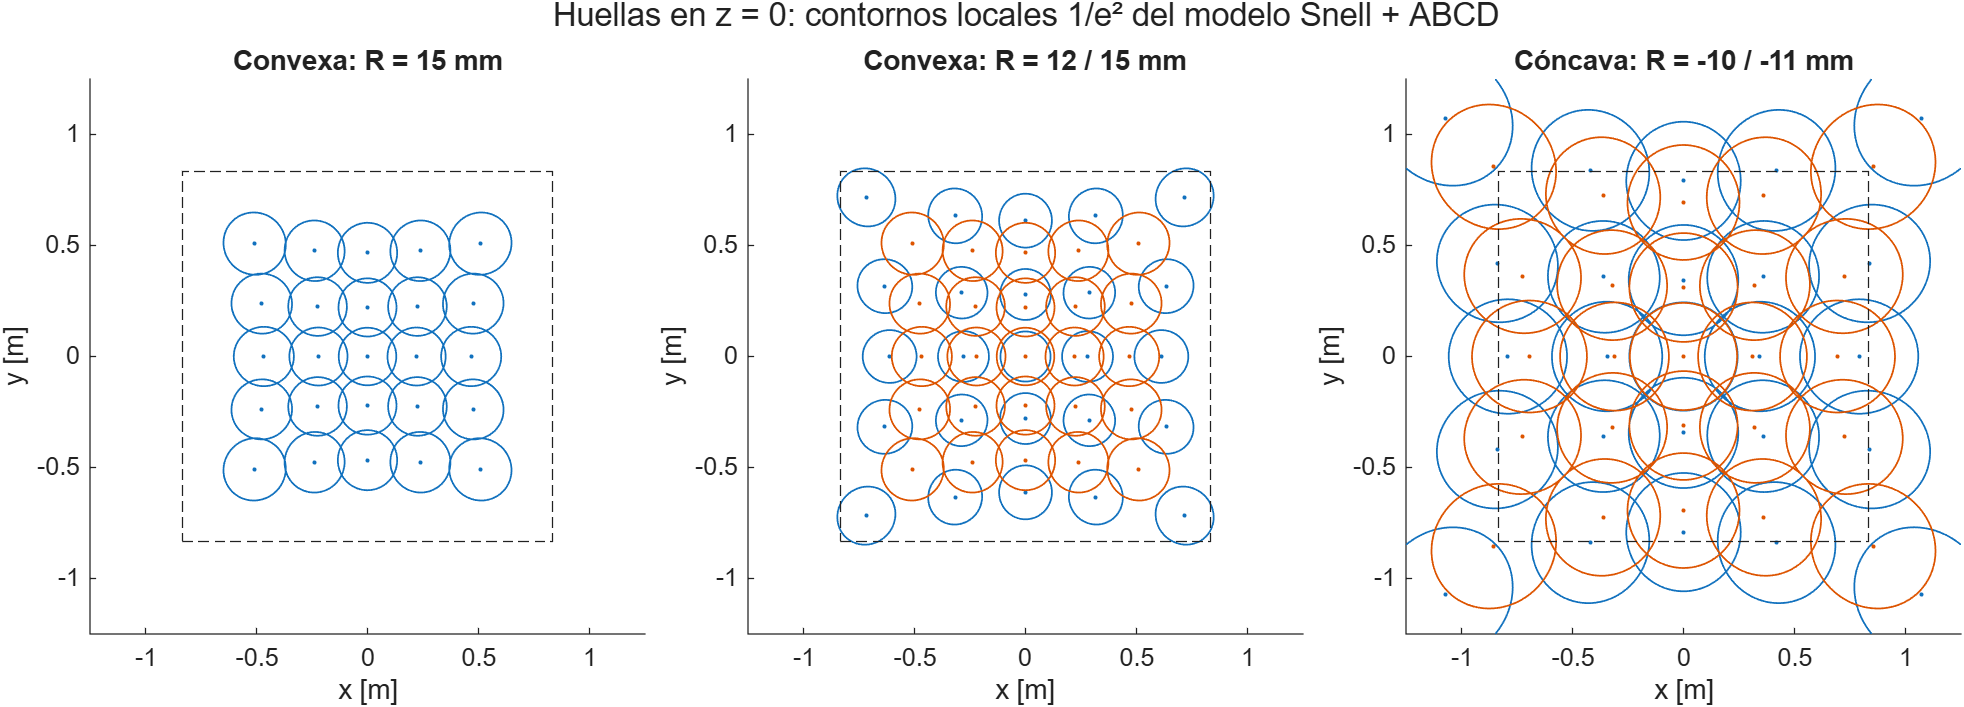
\includegraphics[width=\linewidth]{01_huellas_opticas.png}
\caption{La lente fija separa los haces; demasiada separación deja poca información entre ellos o en los bordes. Dos focales cambian la huella. La familia cóncava aumenta el solapamiento en el modelo inicial, pero su adecuación física debe comprobarse aparte.}
\end{figure}

\begin{figure}[H]\centering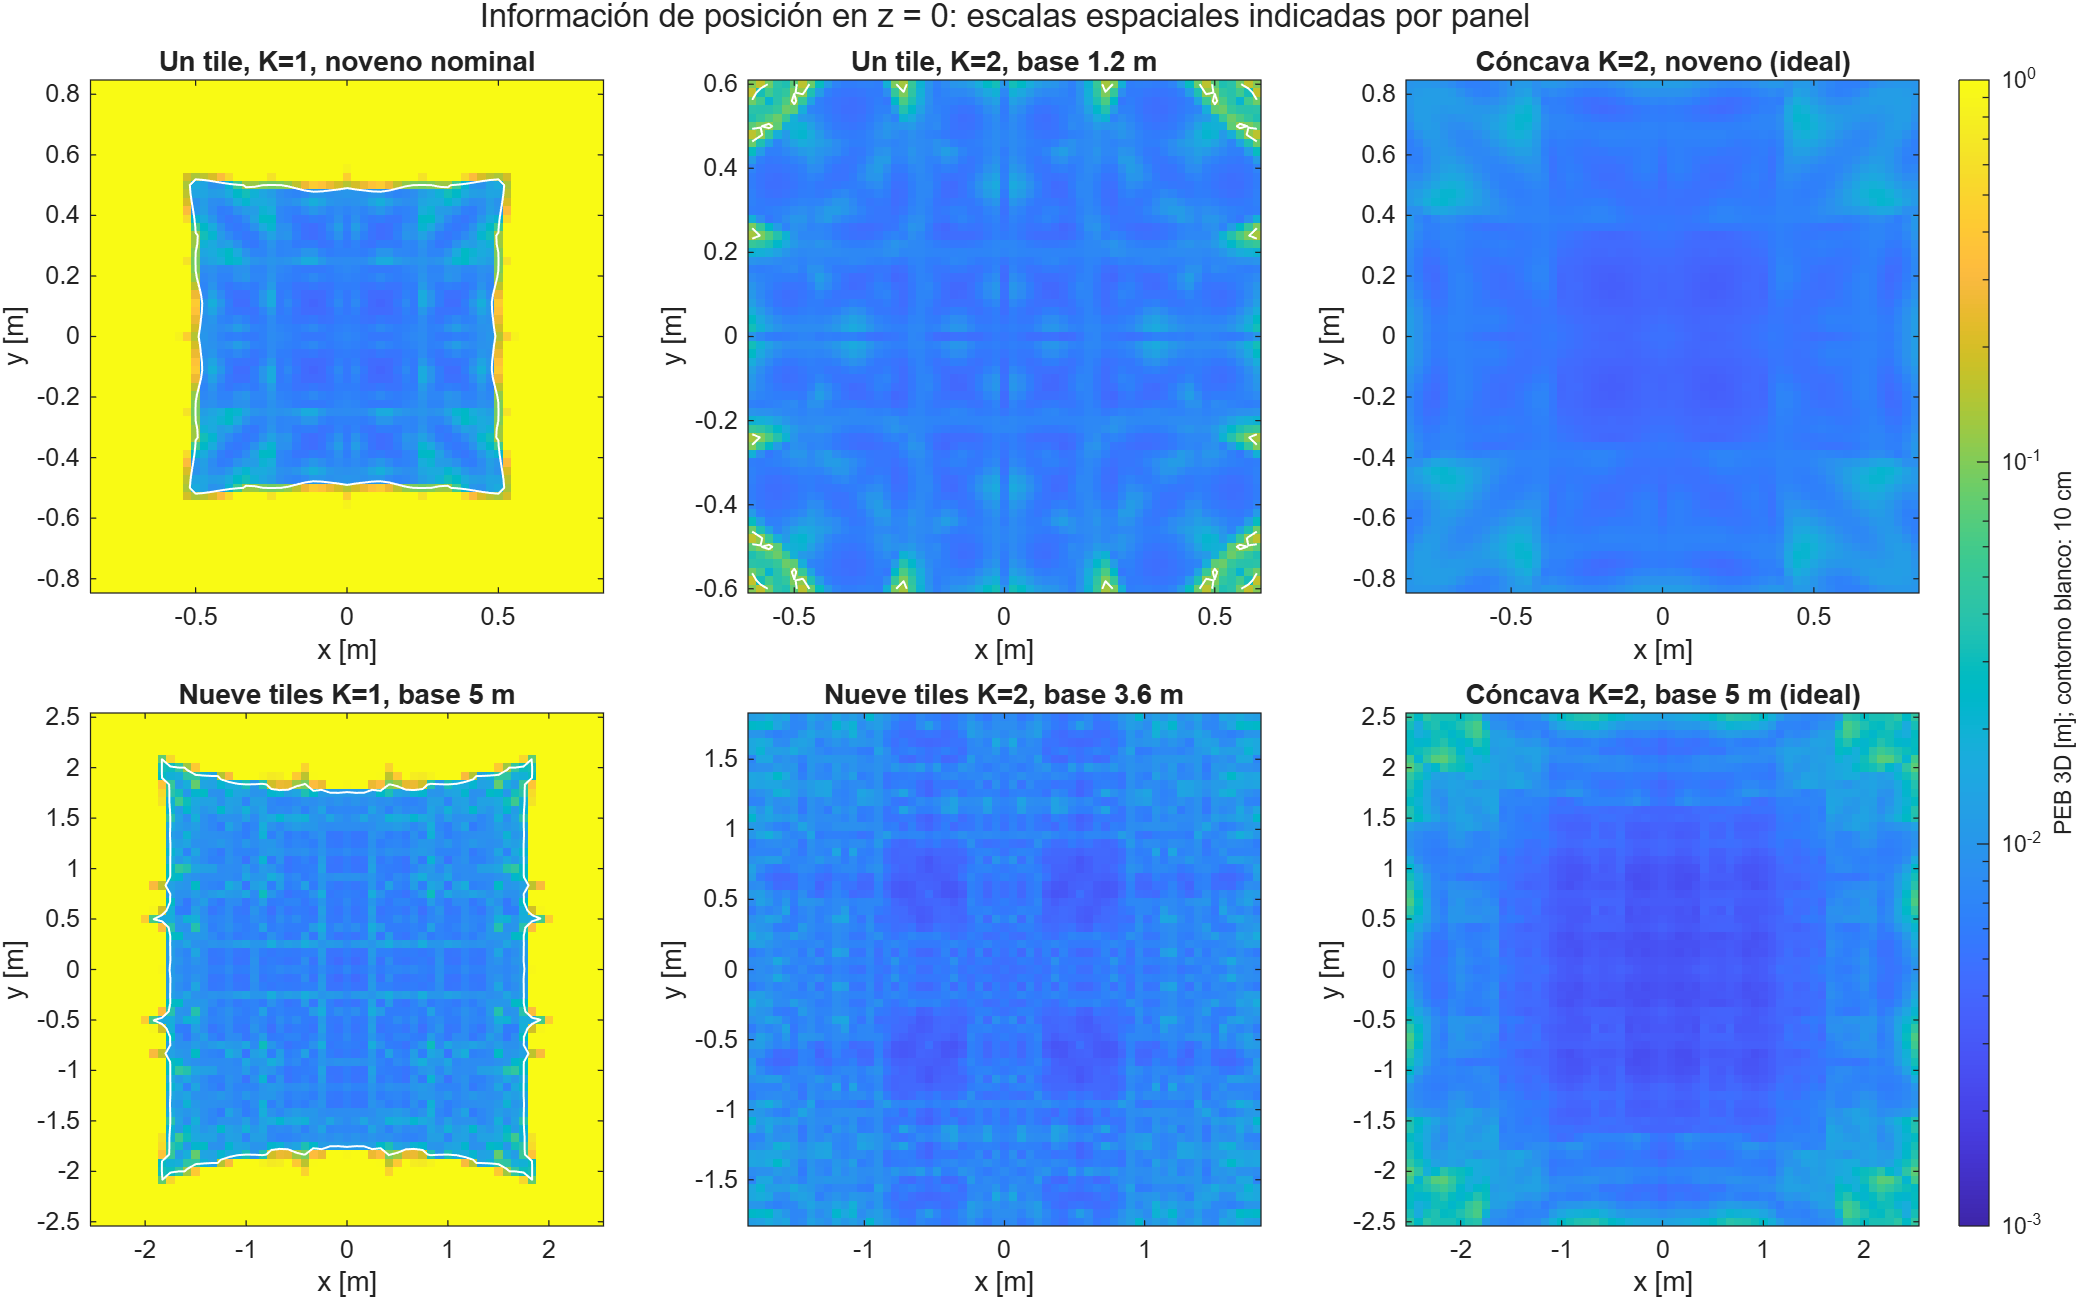
\includegraphics[width=\linewidth]{05_mapas_informacion.png}
\caption{Mapas de información en el plano $z=0$. Las escalas laterales varían entre paneles y se indican en los ejes. Los valores no acotados se representan saturados por encima de la escala, no como precisión nula. Las regiones con buena PEB no son un certificado de unicidad global.}
\end{figure}

\subsection{Distribuciones del error y resultados completos}
Las curvas muestran todo el rango de errores, incluidos valores métricos. Son distribuciones espaciales con ruido, no únicamente repeticiones alrededor de una posición favorable.
\begin{figure}[H]\centering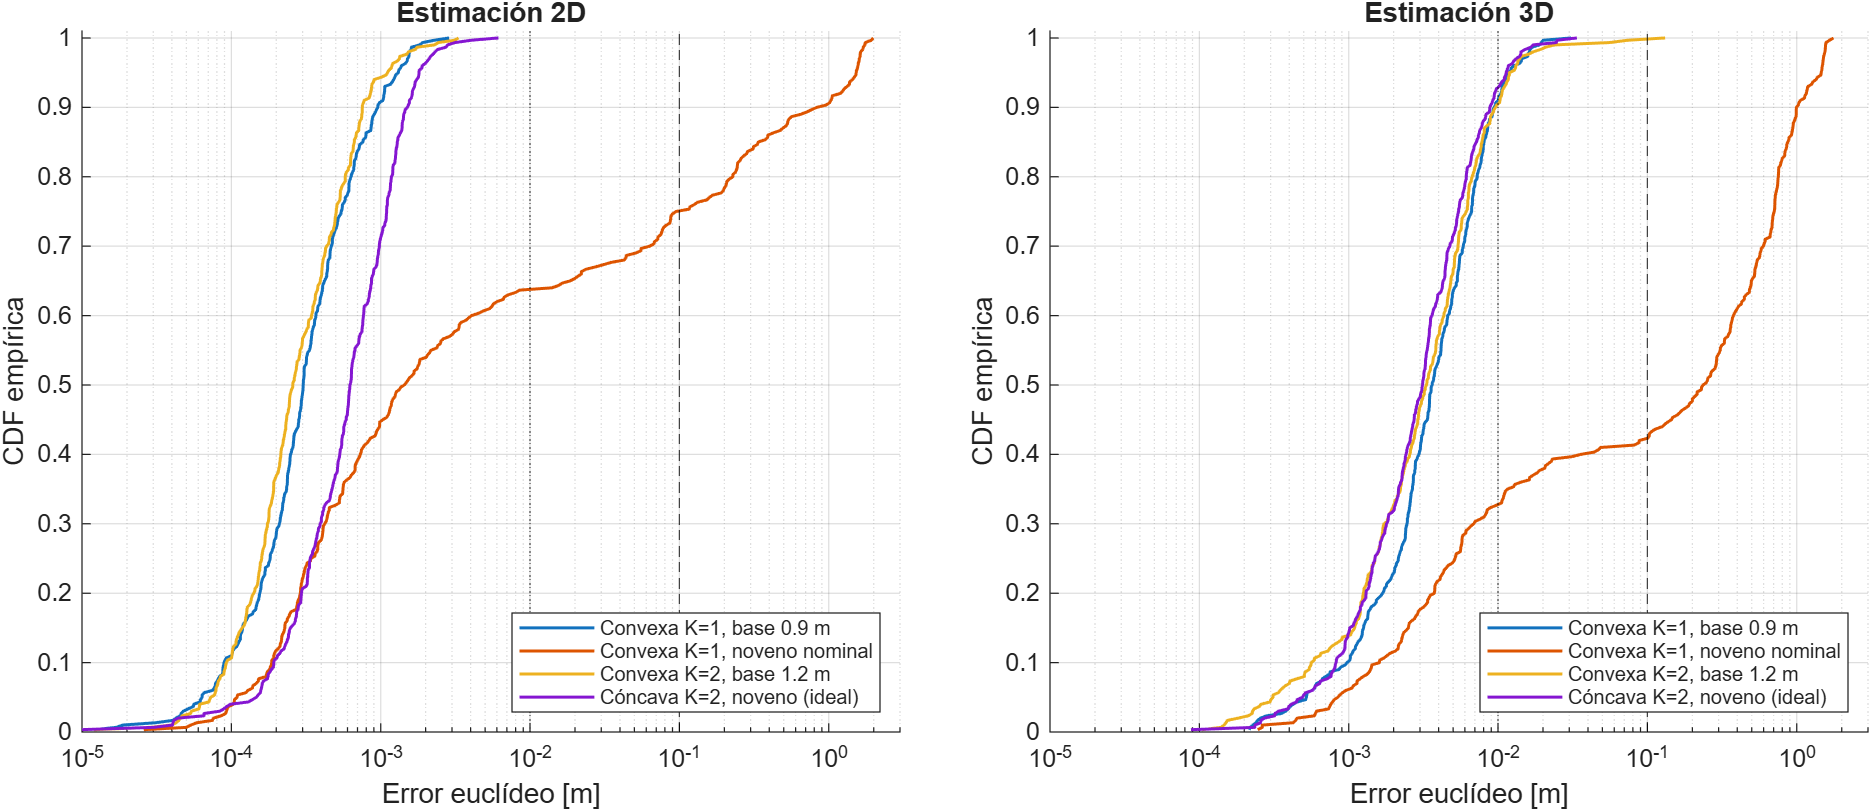
\includegraphics[width=\linewidth]{06_cdf_tile.png}
\caption{Experimentos de un tile. Se comparan dominios declarados distintos, no se afirma que reducir el dominio constituya una mejora óptica. Las líneas de referencia son 1 y 10 cm.}
\end{figure}
\begin{figure}[H]\centering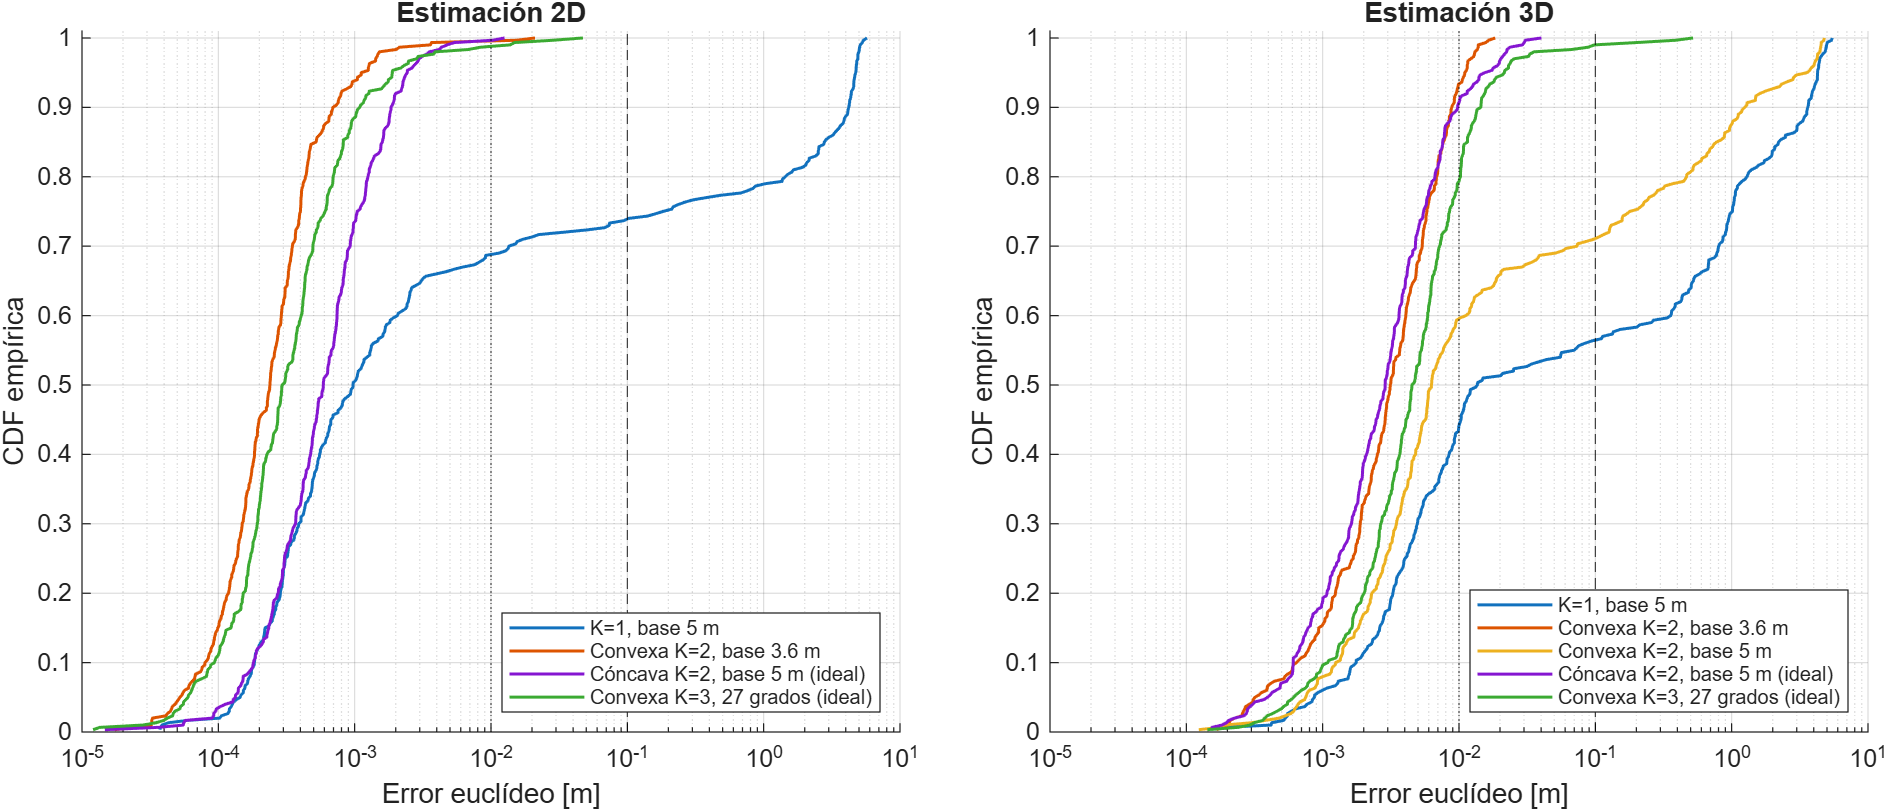
\includegraphics[width=\linewidth]{07_cdf_grid.png}
\caption{Experimentos de nueve tiles. Las etiquetas ``ideal'' identifican variantes cuya buena CDF bajo el modelo circular no constituye una validación física. La base 3.6 m no se confunde con la base nominal de 5 m.}
\end{figure}

\begin{longtable}{lrrrrr}\toprule
ID & Mediana [mm] & P95 [mm] & RMSE [mm] & Máximo [mm] & $<10$ cm [\%]\\\midrule\endhead
C01 & 0.303 & 1.31 & 0.593 & 2.87 & 100 \\
C02 & 3.63 & 11.7 & 6.22 & 30.9 & 100 \\
C03 & 1.46 & 1.53e+03 & 494 & 1.99e+03 & 75 \\
C04 & 242 & 1.46e+03 & 599 & 1.76e+03 & 42 \\
C05 & 0.258 & 1.11 & 0.572 & 3.32 & 100 \\
C06 & 3.33 & 12 & 10.9 & 131 & 99.7 \\
C07 & 0.626 & 1.8 & 1.02 & 6.15 & 100 \\
C08 & 3.13 & 11.3 & 5.79 & 33.7 & 100 \\
C09 & 0.973 & 4.74e+03 & 1.8e+03 & 5.72e+03 & 73.7 \\
C10 & 13.7 & 4.27e+03 & 1.65e+03 & 5.47e+03 & 56.3 \\
C11 & 0.239 & 1.12 & 1.6 & 21 & 100 \\
C12 & 3.15 & 11 & 5.38 & 18.4 & 100 \\
C13 & 0.589 & 2.43 & 1.49 & 12.6 & 100 \\
C14 & 2.87 & 15.6 & 7.12 & 40.2 & 100 \\
C15 & 0.3 & 1.89 & 3.53 & 47.2 & 100 \\
C16 & 4.6 & 21.5 & 41 & 521 & 99 \\
C17 & 12.4 & 810 & 307 & 1.03e+03 & 68.7 \\
C18 & 4.3 & 286 & 135 & 908 & 84 \\
C19 & 6.2 & 56.4 & 29 & 172 & 97.7 \\
C20 & 6.29 & 3.58e+03 & 1.12e+03 & 4.78e+03 & 71 \\
C21 & 3.69 & 25.4 & 15.1 & 111 & 99.7 \\
C22 & 4.59 & 521 & 726 & 4.94e+03 & 86.3 \\
C23 & 431 & 904 & 528 & 1e+03 & 11.7 \\
C24 & 457 & 965 & 560 & 1.03e+03 & 11 \\
C25 & 47.7 & 655 & 286 & 1.37e+03 & 69.3 \\
\bottomrule\end{longtable}

\begin{longtable}{lrrrr}\toprule
ID & Frontera máx. [mm] & P95 PEB [mm] & PEB $<10$ cm [\%] & Rango completo [\%]\\\midrule\endhead
C01 & 1.88 & 1.55 & 100 & 100 \\
C02 & 16.2 & 11.7 & 100 & 100 \\
C03 & 2.18e+03 & 1.42e+09 & 67.6 & 96.9 \\
C04 & 1.85e+03 & $\infty$ & 36 & 81.2 \\
C05 & 7.05 & 1.58 & 99.9 & 100 \\
C06 & 382 & 24.3 & 99.7 & 100 \\
C07 & 1.83 & 1.86 & 100 & 100 \\
C08 & 26 & 9.85 & 100 & 100 \\
C09 & 5.64e+03 & 1.38e+09 & 72.2 & 99.8 \\
C10 & 5.17e+03 & $\infty$ & 53.2 & 93.4 \\
C11 & 3.73 & 1.68 & 100 & 100 \\
C12 & 9.02 & 10.2 & 100 & 100 \\
C13 & 5.71 & 2.74 & 100 & 100 \\
C14 & 74.3 & 19.7 & 100 & 100 \\
C15 & 6.25 & 2.27 & 99.8 & 100 \\
C16 & 769 & 42.7 & 98 & 100 \\
C17 & 1.14e+03 & 2.03e+06 & 63.1 & 97.4 \\
C18 & 1.08e+03 & 2.34e+03 & 74.2 & 99.8 \\
C19 & 58.9 & 58.8 & 98.1 & 100 \\
C20 & 4.64e+03 & 3.78e+08 & 69 & 99.4 \\
C21 & 522 & 206 & 93.3 & 100 \\
C22 & 4.54e+03 & 1.25e+05 & 80.7 & 100 \\
C23 & 1.02e+03 & 3.82e+04 & 0.00537 & 100 \\
C24 & 1.07e+03 & 1.7e+04 & 0 & 100 \\
C25 & 1.54e+03 & 1.31e+04 & 54.1 & 100 \\
\bottomrule\end{longtable}


Las tablas presentan error aleatorio y máximo estructurado por separado. La columna de éxito se refiere a error inferior a 10 cm, no a la bandera de convergencia del optimizador. Los intervalos de Wilson, RMSE por eje y mínimos alternativos se conservan en \archivo{tablas/summary.csv}. Los casos cóncavos se mantienen para documentar el camino explorado, no se seleccionan sin las reservas ópticas siguientes.

\subsection{La ganancia desconocida cambia la conclusión de profundidad}
En el núcleo del tile, liberar una ganancia común eleva el P95 3D a \GananciaLibrePtres{} mm. El AP con varios orígenes puede mejorar algunos puntos, pero no elimina todas las zonas de altura débil. Este resultado concuerda con la invariancia de campo lejano demostrada antes y con las curvas radiales del coste.
\begin{figure}[H]\centering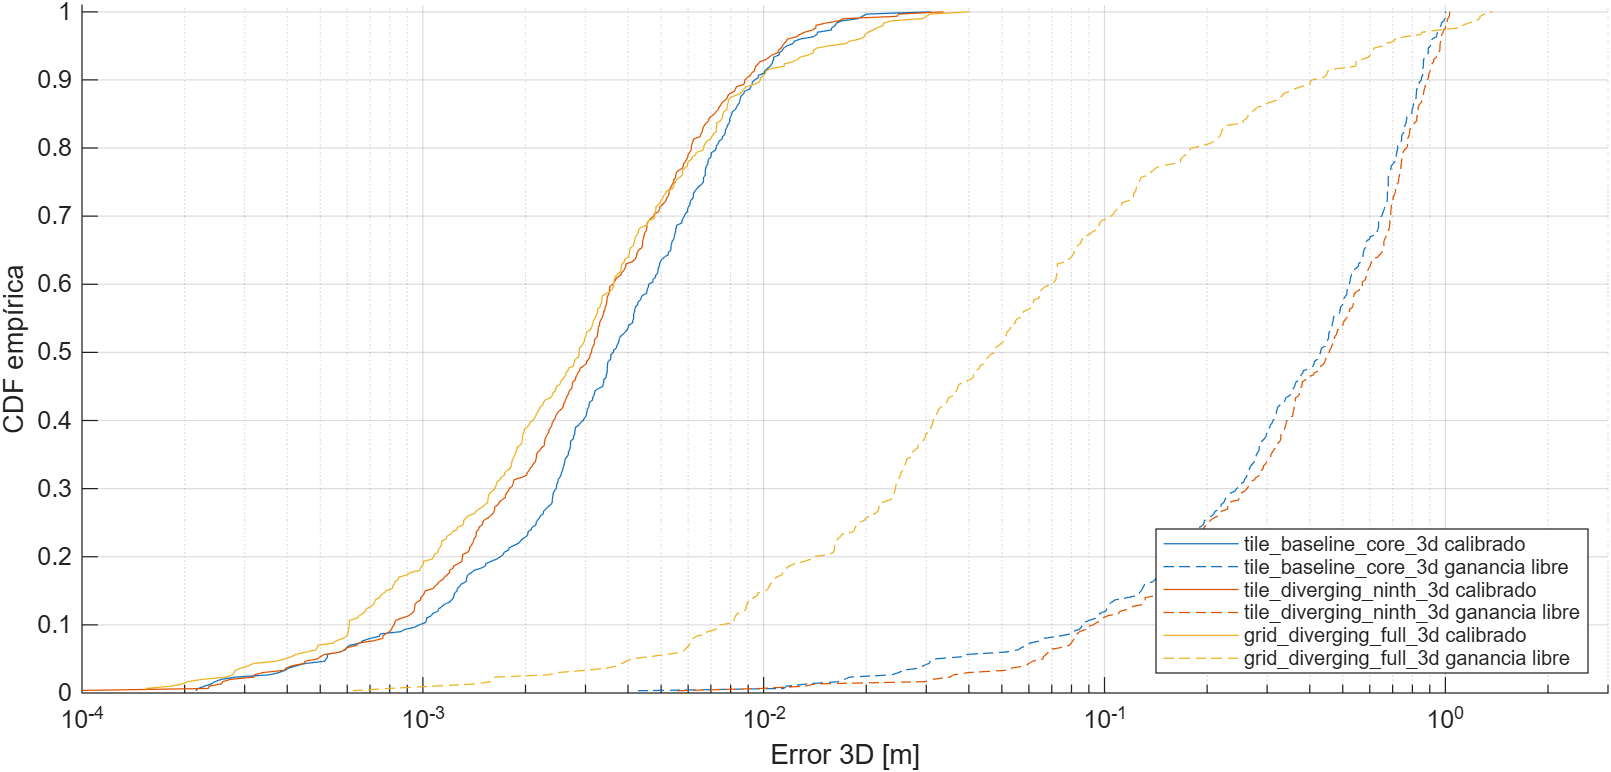
\includegraphics[width=\linewidth]{08_ganancia_desconocida.png}
\caption{Ganancia calibrada frente a ganancia estimada. El mismo color agrupa una geometría; las líneas discontinuas liberan la ganancia. Las diferencias no deben atribuirse a un cambio de número de PDs.}
\end{figure}

\subsection{La calibración importa incluso sin liberar la ganancia}
\begin{table}[H]\centering
\begin{tabular}{lrr}\toprule
Perturbación & P95 [mm] & RMSE [mm]\\\midrule
Control concordante & 10.7 & 5.3 \\
Ganancia +2\% & 35.2 & 25.6 \\
Calibración por VCSEL 1\% & 16.8 & 9.91 \\
Fondo residual 0.1 nW & 33.1 & 16 \\
Inclinación PD $3^\circ$ & 15.7 & 8.32 \\
Curvatura +0.1\% & 18.1 & 10.1 \\
Curvatura +1\% & 121 & 82.6 \\
Borde +0.1 mm & 22.3 & 12.3 \\
\bottomrule\end{tabular}

\caption{Sensibilidad del núcleo del tile, con 100 posiciones por condición. El modelo del estimador permanece nominal. El control tiene una realización distinta de la serie principal de 300 posiciones.}
\end{table}
\begin{figure}[H]\centering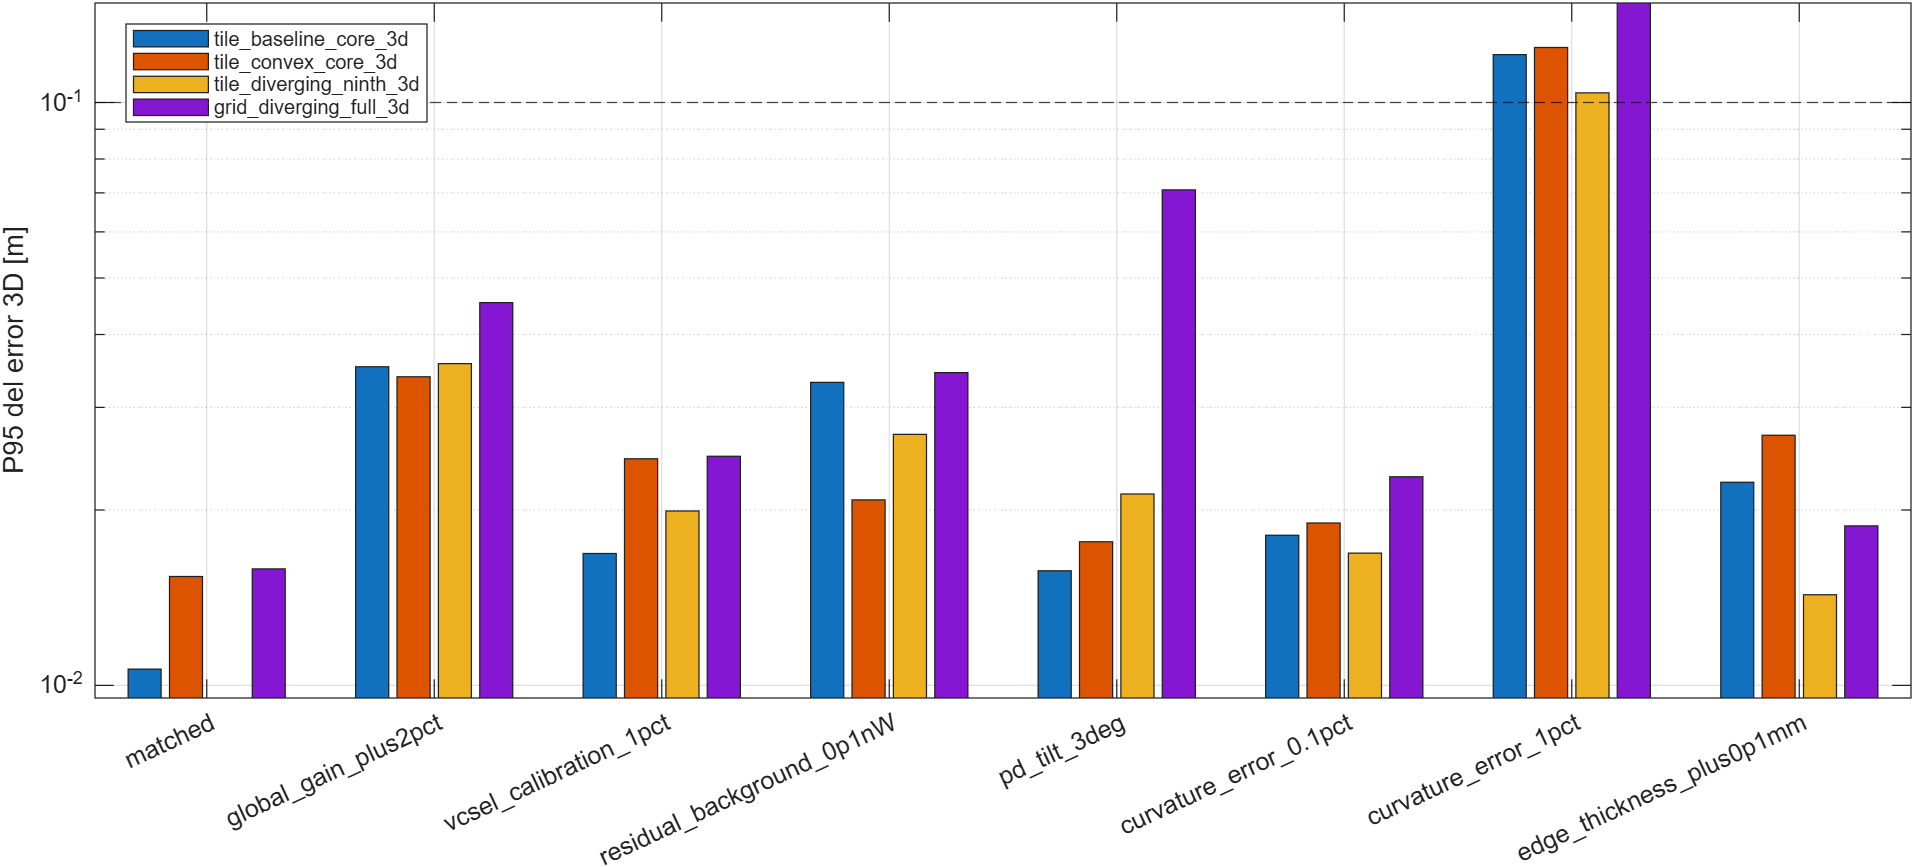
\includegraphics[width=\linewidth]{09_sensibilidad_calibracion.png}
\caption{Errores de ganancia, curvatura, geometría y orientación. Estos ensayos paramétricos no sustituyen una simulación de estimación sobre irradiancias aberradas reales.}
\end{figure}
Un error porcentual de curvatura cambia simultáneamente dirección y ancho. Por eso puede producir sesgos considerablemente mayores que el ruido del caso perfectamente calibrado. Un valor milimétrico de una simulación concordante no equivale a tolerar errores porcentuales de fabricación.

\subsection{Comprobación física: no aceptar una solución solo por su CDF}
\begin{table}[H]\centering
\begin{tabular}{rrrrr}\toprule
$R$ [mm] & Radio menor/ABCD & Radio mayor/ABCD & Centroide [mm] & TIR [\%]\\\midrule
12 & 0.876 & 0.896 & 0.222 & 0 \\
15 & 0.953 & 1.01 & 0.441 & 0 \\
-10 & 1.17 & 2.57 & 65.4 & 2.04 \\
-11 & 1.11 & 1.91 & 34.9 & 0.0235 \\
10 & 0.31 & 0.595 & 1.38 & 0 \\
\bottomrule\end{tabular}

\caption{Emisor de esquina: comparación entre segundos momentos del trazado y la aproximación circular proyectada. Cada fila utiliza 200000 rayos.}
\end{table}
\begin{figure}[H]\centering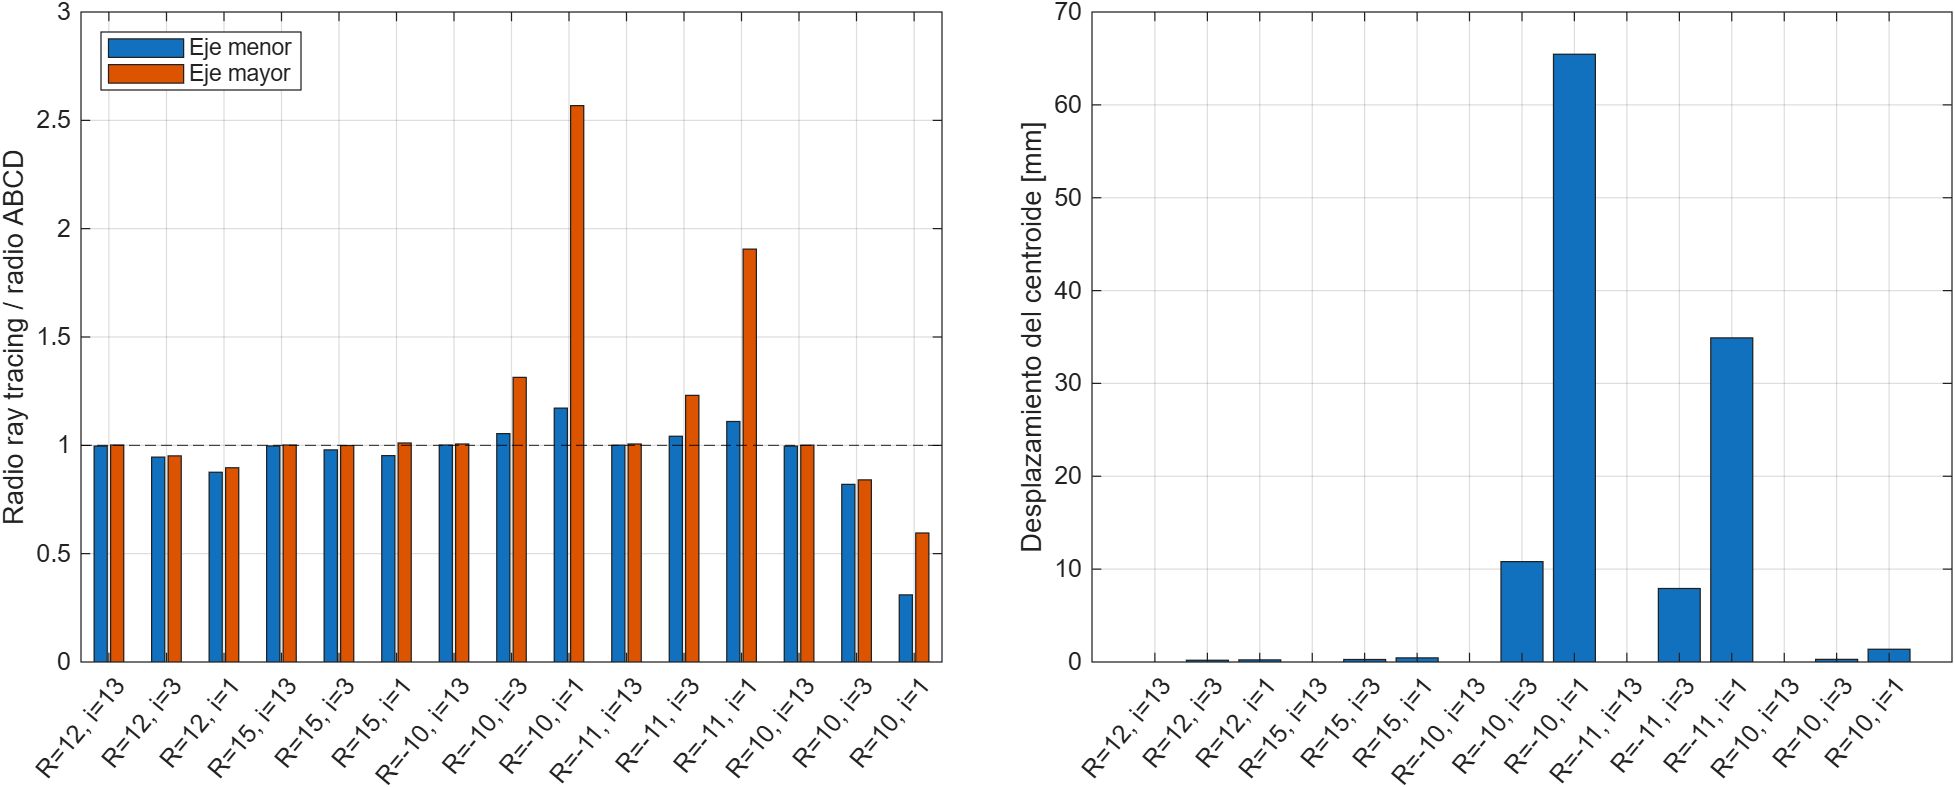
\includegraphics[width=\linewidth]{10_validacion_ray_tracing.png}
\caption{Comparación completa de quince configuraciones. Una razón de radios cercana a uno favorece la aproximación; grandes diferencias o desplazamientos de centroide invalidan una lectura literal de las CDF concordantes.}
\end{figure}
\begin{figure}[H]\centering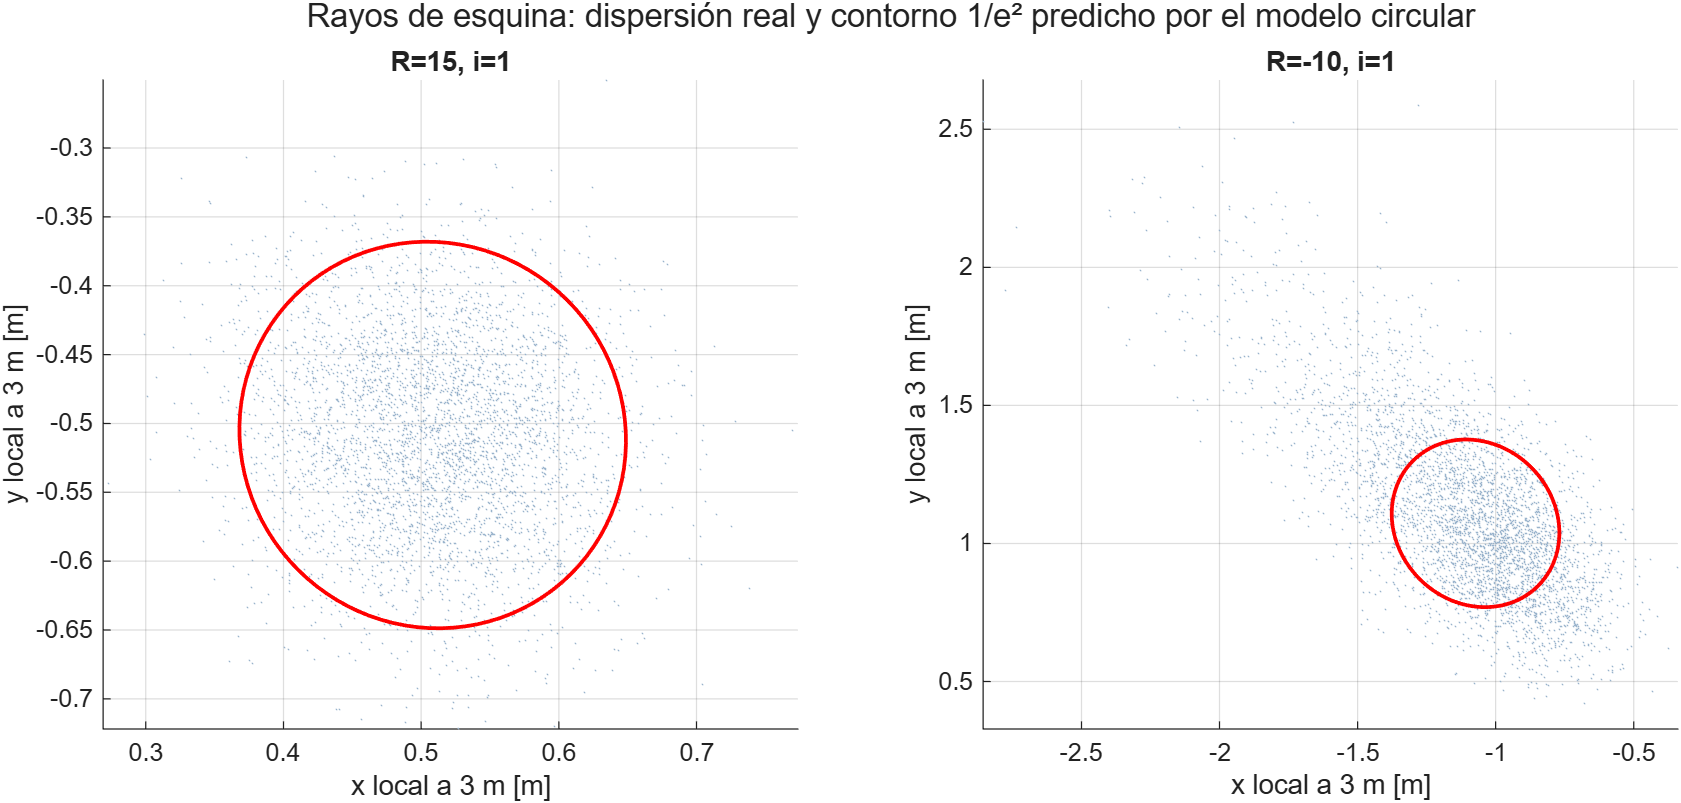
\includegraphics[width=\linewidth]{11_aberraciones_esquina.png}
\caption{Visualización de rayos de esquina y del contorno predicho por el Gaussian circular. El cambio a focal negativa fuerte requiere más que reutilizar un único ancho circular.}
\end{figure}

El estado original $R=15$ mm se mantiene relativamente próximo al modelo de referencia, aunque incluso errores de pocos puntos porcentuales en ancho pueden amplificarse en las colas de potencia. $R=12$ mm también requiere calibración de forma para defender precisión experimental fina. $R=10$ mm y los estados negativos fuertes muestran desviaciones off-axis mucho mayores; puede haber TIR de parte de los rayos aunque el rayo principal se transmita.

\textbf{Decisión:} las variantes cóncava y de tres estados con reajuste a $27^\circ$ son rutas exploratorias, no recomendaciones validadas por este informe. Antes de adoptarlas deben usarse un modelo astigmático/no paraxial o firmas medidas y repetirse toda la evaluación. No se ha efectuado una estimación extremo a extremo usando un receptor real ni se demuestra el rendimiento bajo aberraciones reales con las cifras del modelo concordante.

\subsection{Tiempo, área y complejidad}
\begin{figure}[H]\centering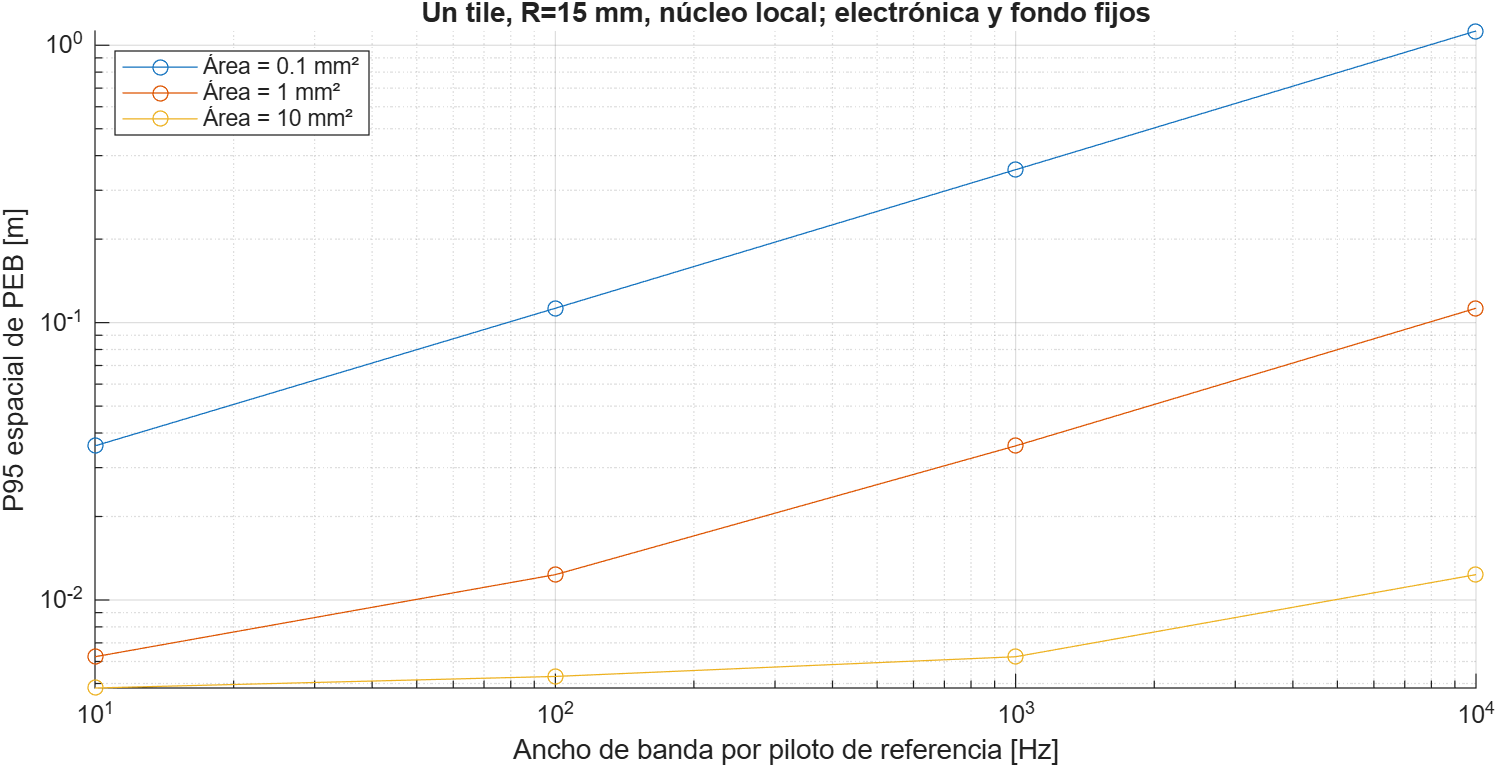
\includegraphics[width=.88\linewidth]{12_tiempo_area_ruido.png}
\caption{Sensibilidad del núcleo de un tile al área y a la banda de medida. Aumentar banda acorta integración. Se mantiene fija la electrónica y la corriente de fondo, por lo que no se está diseñando la capacitancia ni el amplificador de un PD mayor.}
\end{figure}

Los barridos de pitch y de muchos estados se conservan completos. No se observa una regla universal ``más separación o más K es mejor'': separar haces aumenta cobertura angular, pero puede reducir solapamiento detectable. Los controles de repetición indican qué parte de una mejora procede solo de promediado. El resultado práctico favorece empezar por una focal y una región útil delimitada.

\begin{figure}[H]\centering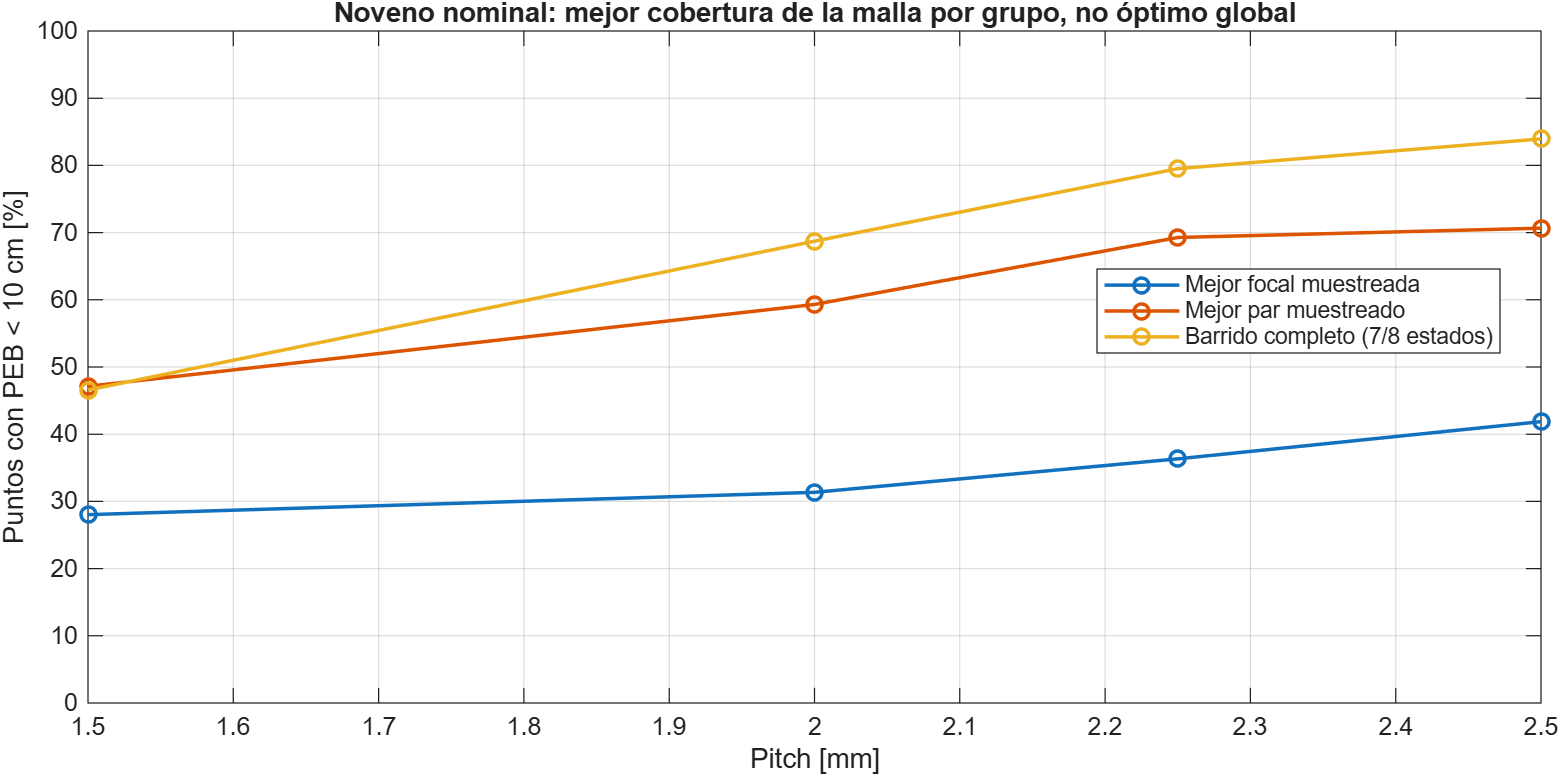
\includegraphics[width=.9\linewidth]{13_barrido_pitch.png}
\caption{Mejor fracción de puntos con PEB inferior a 10 cm entre los estados muestreados de cada grupo, en el noveno nominal. La selección procede de una malla finita: no es un óptimo global ni una garantía de cobertura continua.}
\end{figure}
\begin{figure}[H]\centering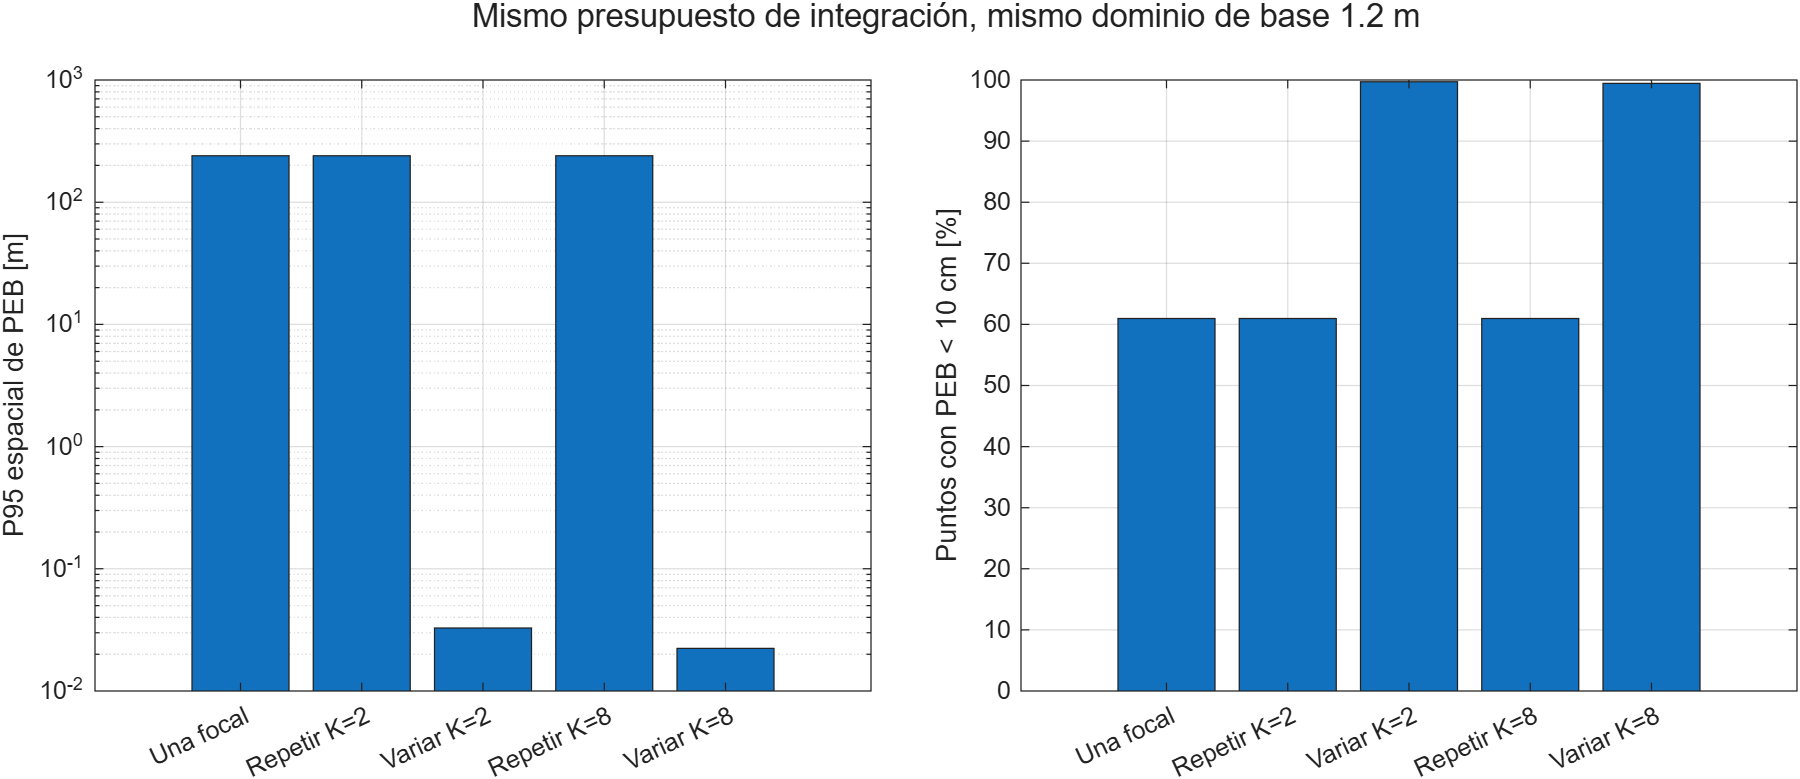
\includegraphics[width=\linewidth]{14_repeticion_vs_diversidad.png}
\caption{Repetir la misma focal frente a variar la curvatura, con el mismo dominio y presupuesto de integración. Promediar fluctuaciones independientes no equivale a generar gradientes espaciales nuevos.}
\end{figure}
\begin{figure}[H]\centering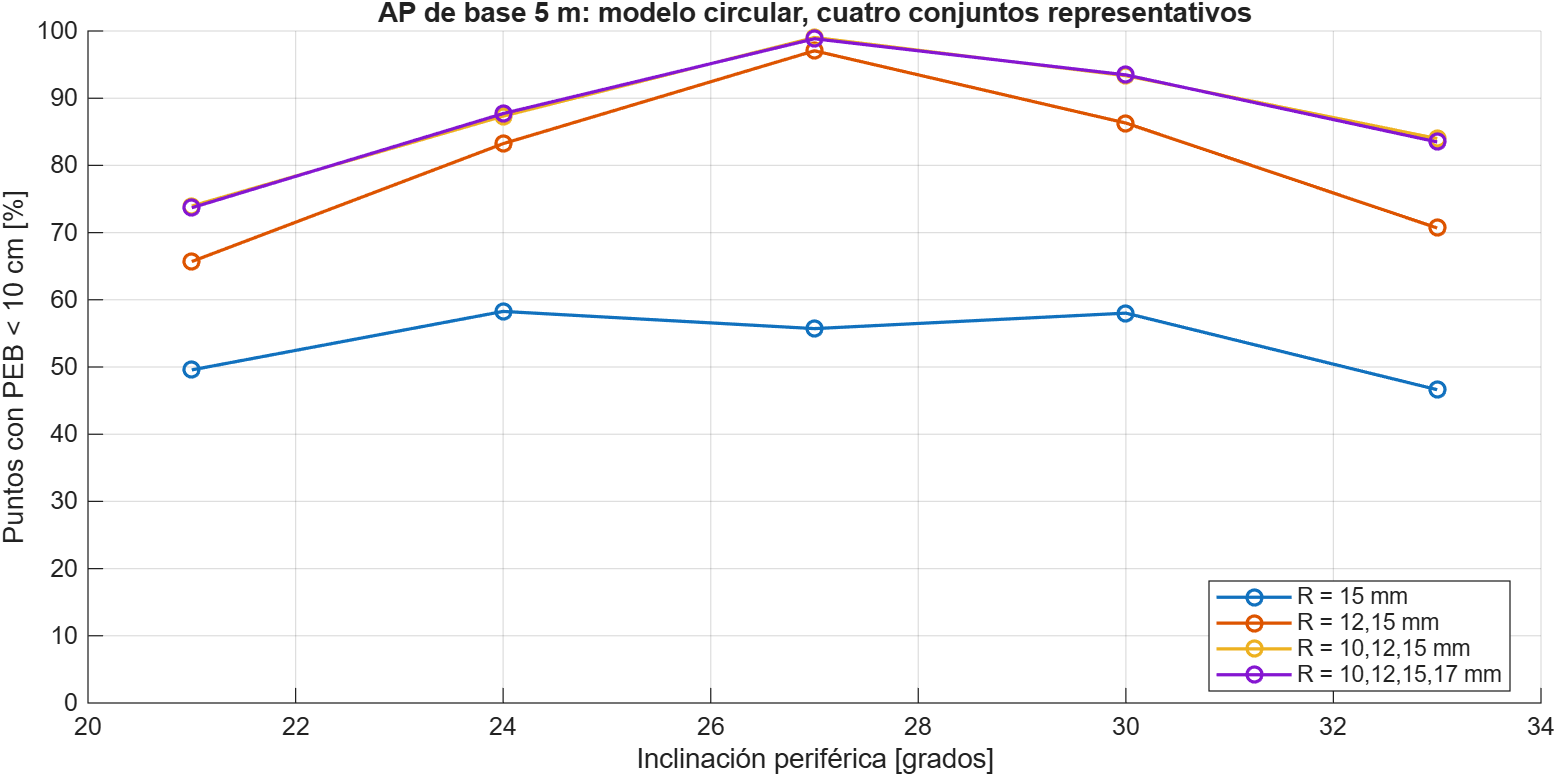
\includegraphics[width=.9\linewidth]{15_barrido_inclinacion.png}
\caption{Inclinación de los tiles periféricos y fracción de puntos localmente favorables del AP. Se muestran cuatro de los seis conjuntos de estados para facilitar la lectura; todos se conservan en CSV. Los conjuntos con R=10 mm siguen sujetos a la advertencia de aberraciones.}
\end{figure}

\subsection{Relación con las cifras Python}
\begin{table}[H]\centering\begin{tabular}{p{6.6cm}rr}\toprule
Caso & P95 Python [mm] & P95 MATLAB [mm]\\\midrule
\path{tile_baseline_core_3d} & 12.2 & 11.7 \\
\path{tile_convex_core_3d} & 17.9 & 12 \\
\path{grid_convex_core_3d} & 13.8 & 11 \\
\path{tile_baseline_ninth_3d} & 1.31e+03 & 1.46e+03 \\
\bottomrule\end{tabular}\caption{Comparación de realizaciones independientes, no equivalencia muestra a muestra.}\end{table}

La comparación anterior es estadística, no una prueba de igualdad muestra a muestra. Los generadores son distintos y \archivo{lsqnonlin} no usa exactamente el criterio de parada de SciPy. La equivalencia determinista se comprueba por separado con cinco configuraciones y ocho posiciones cada una: salidas, direcciones, $q$, potencias, Jacobianos e información en puntos numéricamente estables. Los puntos oscuros permanecen en los mapas y las estadísticas; no se omiten para forzar equivalencia de covarianzas mal condicionadas.

\subsection{Recomendación final y límites de aplicabilidad}
\begin{enumerate}
\item Empezar por un tile, pitch 2 mm y $R=15$ mm, con normal y potencia absoluta calibradas.
\item Utilizar el vector de emisores identificados y el ajuste conjunto, no solo el índice del haz máximo ni la suma.
\item Añadir el estado $R=12$ mm si se necesita ampliar la región, después de calibrar su patrón off-axis.
\item Para nueve tiles, mantener explícita la región útil; no prometer automáticamente 25 m$^2$ ni todo un prisma de altura variable.
\item No confundir ganancia desconocida con una fluctuación pequeña: cambia fundamentalmente la observabilidad de distancia.
\end{enumerate}

No se ha identificado ni certificado una lente comercial que reproduzca simultáneamente curvatura, apertura, espesor y dinámica supuestos. Los estados convexos moderados requieren aproximadamente 36.67 y 45.83 dioptrías sobre 16 mm; los cóncavos exploratorios, $-50$ y $-55$ dioptrías. La repetibilidad, histéresis y aberraciones son parte de la verificación experimental pendiente. Los 10 mW se adoptan del contexto del artículo, pero no certifican seguridad ocular de los estados o transitorios modificados. Todas las pruebas de este informe son computacionales.

\section{Organización, depuración y reproducción}
\subsection{Qué abrir primero}
\begin{enumerate}
\item Leer este PDF: \archivo{informe/compilado/INFORME.pdf}.
\item Abrir \archivo{demo_localizacion.m} para recorrer manualmente la cadena parámetros $\to$ óptica $\to$ potencias $\to$ ruido $\to$ estimación $\to$ error.
\item Abrir \archivo{configuracion/gob_config.m} y \archivo{configuracion/gob_noise.m} para identificar las hipótesis numéricas.
\item Abrir un archivo MAT de \archivo{ensayos/} y la figura FIG correspondiente para inspeccionar resultados concretos.
\end{enumerate}

\subsection{Mapa de archivos y relación con el razonamiento}
Todas las rutas de esta tabla son relativas a \archivo{simulation_MATLAB}.
\begin{longtable}{p{6.1cm}p{8.4cm}}\toprule
Archivo o carpeta & Función en el estudio\\\midrule\endhead
\archivo{run_gob.m} & Punto de entrada. Modos demo, test, quick, full, plots, verify y report. Crea directorios fechados y rechaza sobreescrituras de ejecuciones.\\
\archivo{gob_paths.m} & Añade únicamente las carpetas de este estudio al path; no importa árboles ajenos del repositorio.\\
\archivo{demo_localizacion.m} & Script de depuración con nombres de variables en español y resultados en Workspace.\\
\archivo{configuracion/gob_config.m} & Dimensiones, potencias, lente, pitch, tiles y PD.\\
\archivo{configuracion/gob_noise.m} & Electrónica, ruido y fluctuación por piloto.\\
\archivo{configuracion/gob_study_cases.m} & Catálogo de los 25 problemas y dominios.\\
\archivo{configuracion/gob_run_options.m} & Semillas, resolución, número de ensayos y selección de experimentos.\\
\archivo{modelo/gob_model.m} & Superficie, Snell de rayos principales, ABCD, montaje y etiquetas.\\
\archivo{modelo/gob_power.m} & Potencias, Jacobiano y variables geométricas intermedias de cada haz.\\
\archivo{modelo/gob_sigma.m} & Desviación de medida en W.\\
\archivo{modelo/gob_rotation.m} & Rotaciones de los tiles.\\
\archivo{modelo/gob_footprints.m} & Intersección de ejes con un plano receptor.\\
\archivo{modelo/gob_diagnostics.m} & Focales, espesores, waists y clipping para auditar parámetros.\\
\archivo{modelo/gob_snell.m} & Snell vectorial usado por el trazador independiente.\\
\archivo{estimacion/gob_information.m} & Información por SVD y eliminación de ganancias nuisance.\\
\archivo{estimacion/gob_estimator.m} & Biblioteca y opciones del ajuste MATLAB.\\
\archivo{estimacion/gob_candidate_costs.m} & Coste de candidatos y ganancia inicial perfilada.\\
\archivo{estimacion/gob_residual.m} & Residuo ponderado y Jacobiano que recibe lsqnonlin.\\
\archivo{estimacion/gob_fit.m} & Arranques múltiples, ajuste y mínimos alternativos.\\
\archivo{estimacion/gob_localize.m} & Función de uso directo con vector de potencias o CSV en W.\\
\archivo{experimentos/gob_run_case.m} & Mapas, datos aleatorios, fronteras y auditoría de un caso.\\
\archivo{experimentos/gob_sample_positions.m} & Muestreo uniforme en volumen demostrado en el informe.\\
\archivo{experimentos/gob_metric_grid.m} & Malla de información del dominio declarado.\\
\archivo{experimentos/gob_boundary_positions.m} & Fronteras, ejes y centro, separados de Monte Carlo.\\
\archivo{experimentos/gob_bound_summary.m} & Estadísticas de información que no ocultan infinitos.\\
\archivo{experimentos/gob_design_sweep.m} & Barridos de parámetros y candidatos de diseño.\\
\archivo{experimentos/gob_controls.m} & Repetición, ganancia, inclinación, área y ambigüedad radial.\\
\archivo{experimentos/gob_robustness.m} & Errores sistemáticos de calibración y geometría.\\
\archivo{experimentos/gob_ray_validation.m} & Quince comparaciones de rayos, tablas y ejemplos.\\
\archivo{validacion/gob_trace_beam.m} & Propagación geométrica independiente de las fórmulas ABCD.\\
\archivo{validacion/gob_verify_results.m} & Recalcula estadísticas, comprueba coordenadas de mapas, medias, tablas y conservación de Python.\\
\archivo{validacion/gob_rebuild_maps.m} & Regenera mapas y columnas de información desde el manifiesto sin alterar observaciones ni estimaciones guardadas.\\
\archivo{validacion/gob_audit_solver.m} & Reajusta el peor ensayo guardado con tres combinaciones de malla y arranques, conservando explícito el error original.\\
\archivo{validacion/gob_export_python_reference.m} & Extracción opcional de referencias Python, solo para auditar la migración.\\
\archivo{validacion/gob_python_snapshot.m} & Inventario de hashes para verificar la conservación del trabajo anterior.\\
\archivo{pruebas/} & Pruebas de modelo, estimador, referencias y convenciones de importación.\\
\archivo{graficas/gob_plot_optics.m} & Geometría, huellas, evolución Gaussian y superficies de coste.\\
\archivo{graficas/gob_plot_results.m} & Mapas, CDF, sensibilidad, rayos y compromiso de adquisición.\\
\archivo{graficas/gob_plot_design.m} & Comparaciones de pitch, repetición de estados e inclinación.\\
\archivo{graficas/gob_save_figure.m} & Exportación PNG, PDF vectorial y FIG editable.\\
\archivo{utilidades/gob_grid.m} & Orden cartesiano compatible con el catálogo de canales y tratamiento de una única muestra.\\
\archivo{utilidades/gob_quantile.m} & Convenciones explícitas de percentiles y cuantiles ordenados.\\
\archivo{utilidades/gob_error_summary.m} & RMSE, percentiles y Wilson.\\
\archivo{utilidades/gob_read_table.m} & Importación tipada: una lista de radios no se interpreta como separador de miles.\\
\archivo{utilidades/gob_update.m}, \archivo{utilidades/gob_merge.m} & Configuración validada y combinación de resultados.\\
\archivo{utilidades/gob_report_tables.m} & Genera tablas y cifras LaTeX directamente desde los resultados MATLAB verificados.\\
\archivo{compilar_informe.m} & Regenera tablas y compila el PDF desde MATLAB.\\
\archivo{informe/} & Fuente LaTeX organizada por capítulos, tablas generadas y PDF compilado.\\
\archivo{referencias/} & Referencias deterministas de migración; no resultados nuevos atribuidos a MATLAB.\\
\archivo{resultados/} & Ejecuciones fechadas, con datos y figuras de MATLAB.\\\bottomrule
\end{longtable}

\subsection{Estructura interna de una ejecución}
\begin{itemize}
\item \archivo{manifest.mat}: casos, opciones, entorno y estado de finalización.
\item \archivo{tablas/summary.csv}: resultados completos de todos los casos; las otras tablas corresponden a controles, diseño, rayos y sensibilidad.
\item \archivo{ensayos/<caso>.mat}: verdad, medias sin ruido, medidas, estimaciones, ganancias, costes, banderas de convergencia y mínimos alternativos.
\item \archivo{ensayos/<caso>_auditoria.mat}: recuperación sin ruido y distancias de firmas a candidatos lejanos.
\item \archivo{mapas/<caso>.mat}: puntos, PEB, desviaciones por eje, valores singulares, rango, número de señales detectables y configuración.
\item \archivo{datos/}: realizaciones completas de sensibilidad, configuraciones de diseño y ejemplos del trazador.
\item \archivo{figuras/}: quince familias de figuras en PNG, PDF y FIG.
\item \archivo{verification.mat}: comprobación de consistencia de la ejecución final.
\end{itemize}
El archivo \archivo{resultados/ultimo_completo.mat} indica la última ejecución completa verificada. Las ejecuciones quick son controles de integración, no resultados de precisión publicables. La documentación no utiliza sus tablas en lugar de las del estudio completo.

\subsection{Cómo ejecutar y depurar en MATLAB}
Desde la raíz del repositorio:
\begin{lstlisting}
addpath('Grid_of_Beams/simulation_MATLAB');
gob_paths;
run_gob('test');
run('Grid_of_Beams/simulation_MATLAB/demo_localizacion.m');
resultado = run_gob('quick');
resultado = run_gob('full');
\end{lstlisting}
Para recorrer la óptica y el ajuste paso a paso:
\begin{lstlisting}
dbstop in gob_power
dbstop in gob_fit
dbstop in gob_residual
\end{lstlisting}
En el script de demostración pueden inspeccionarse \archivo{modelo_optico.origins}, \archivo{modelo_optico.directions}, \archivo{modelo_optico.q}, \archivo{geometria_haces}, \archivo{potencias_medidas_W} y \archivo{resultado.candidate_states}. El modelo no depende de un módulo Python oculto.

Un experimento seleccionado, sin ejecutar el resto:
\begin{lstlisting}
opciones = struct('case_filter',string('tile_convex_core_3d'), ...
    'trials',50,'resolution',21,'sweeps',false,'controls',false, ...
    'rays',false,'robustness',false,'export_figures',false);
resultado = run_gob('full',opciones);
\end{lstlisting}
Se crea otra carpeta fechada. El argumento \archivo{output_directory} permite elegir una ruta nueva explícita, pero se rechaza una carpeta ya existente. Para volver a dibujar y verificar el estudio de referencia:
\begin{lstlisting}
run_gob('plots');
run_gob('verify');
run_gob('report');
\end{lstlisting}
El modo report regenera las tablas LaTeX desde los datos MATLAB, sin recalcular Monte Carlo. Para abrir una figura editable:
\begin{lstlisting}
s = load('Grid_of_Beams/simulation_MATLAB/resultados/ultimo_completo.mat');
openfig(fullfile(s.output_directory,'figuras','06_cdf_tile.fig'));
\end{lstlisting}

Para medidas propias, todas las potencias deben estar en W, identificadas y con el fondo sustraído:
\begin{lstlisting}
y_W = readmatrix('medidas_nW.csv')*1e-9;
solucion = gob_localize('tile_baseline_core_3d',y_W);
\end{lstlisting}
Se deben suministrar 25, 50, 225 o el número que corresponda al caso, en el orden estado/tile/VCSEL. Una potencia agregada no es equivalente. La salida no es fiable automáticamente por el mero hecho de converger.

\subsection{Verificación de la migración y peculiaridades MATLAB}
El entorno verificado es MATLAB R2026a con Optimization Toolbox para \archivo{lsqnonlin}. Los cálculos no requieren Statistics ni Parallel Computing Toolbox. Se emplea \archivo{pagesvd}, por lo que no se afirma compatibilidad con versiones anteriores a su disponibilidad.

Se han aprobado \NumeroPruebas{} pruebas automáticas. Entre ellas se incluyen Snell, normalización de potencia, expresiones cerradas de ABCD, Jacobiano por diferencias finitas, FoV, orden de canales, ganancia nuisance, regiones oscuras, comparación determinista Python y la regresión del inicializador. La comprobación de resultados vuelve a calcular estadísticas desde archivos MAT y comprueba las coordenadas de los mapas, no solo su número de filas.

Dos diferencias de lenguaje requirieron atención explícita:
\begin{enumerate}
\item \archivo{linspace(a,b,1)} devuelve el extremo final en MATLAB, mientras que NumPy devuelve el inicial. Se añadió una prueba de regresión que exige que un mapa 2D esté realmente en $z=0$ y se regeneraron los mapas afectados. Las observaciones y estimaciones 2D, que ya fijaban $z=0$ explícitamente, no dependían de ese error de malla.
\item La inferencia automática de tipos de CSV puede interpretar ``12,15'' como un número con separador de miles. Se fuerza el tipo texto de las listas de radios y se comprueba con una prueba de ida y vuelta.
\end{enumerate}
También se adaptaron los índices desde cero a uno, el orden de almacenamiento por columnas y la definición de percentiles. Estas comprobaciones son parte de una migración científica, no únicamente una traducción literal de operadores.

\subsection{Compilar el informe}
Con TeX Live y desde \archivo{simulation_MATLAB/informe}, después de regenerar tablas:
\begin{lstlisting}[language={}]
pdflatex -interaction=nonstopmode -halt-on-error -output-directory=compilado INFORME.tex
pdflatex -interaction=nonstopmode -halt-on-error -output-directory=compilado INFORME.tex
\end{lstlisting}
Después de cambios de paginación o tablas largas puede ser necesario repetir un tercer pase. La función MATLAB \archivo{compilar_informe} realiza tres pasadas y devuelve la ruta del PDF. Las figuras se leen de la ejecución indicada en \archivo{generado/macros.tex}. La fuente principal está dividida en siete capítulos para que las demostraciones y el relato puedan revisarse independientemente del código.

\subsection{Lista final de interpretación correcta}
\begin{itemize}
\item Un PD no implica una observación escalar si los emisores y estados se identifican por separado.
\item La altura del caso calibrado procede en gran medida de escala radiométrica, no de una firma axial independiente creada necesariamente por la focal.
\item Una PEB pequeña, rango completo y convergencia son comprobaciones diferentes; ninguna sustituye por sí sola la validación completa.
\item Los éxitos locales no son cobertura uniforme del noveno nominal ni de todo el prisma de la habitación.
\item Las mejores CDF del modelo circular no autorizan ignorar aberraciones, calibración ni seguridad ocular.
\end{itemize}

\end{document}
